\documentclass[journal,twoside]{IEEEtran}
\usepackage{cite}
\usepackage{amsmath,amssymb,amsfonts}
%\usepackage{algorithmic}
\usepackage{algorithm}
\usepackage{algpseudocode}
\usepackage{booktabs}
\usepackage{graphicx}
\usepackage{textcomp}
\usepackage{multirow}
\usepackage{adjustbox}
\usepackage{array}
\usepackage{xcolor}
\usepackage{pdflscape}
\usepackage{tabularx}
\usepackage{subcaption}
\usepackage{url}


\def\BibTeX{{\rm B\kern-.05em{\sc i\kern-.025em b}\kern-.08em
    T\kern-.1667em\lower.7ex\hbox{E}\kern-.125emX}}
\markboth{Journal of Modern Power Systems and Clean Energy, VOL. XX, NO. XX, XXXX}
{Author \MakeLowercase{\textit{et al.}}: Preparation of Papers for Journal of Modern Power Systems and Clean Energy}

\begin{document}

\title{Application of the Laplacian Salp Swarm Algorithm to Continuous Wind Farm Layout Optimization}
\author{Prince Solanki, Pulkit Dwivedi, Vanita Garg, and Vinay Shukla
%\thanks{This work has not received any financial support.}
\thanks{Prince Solanki is associated to Department of Mathematics, School of Sciences, IILM University, Greater Noida, Uttar Pradesh, India. Prior to this position, he was at the Department of Mathematics, Indian Institute of Technology, Roorkee, India (e-mail: prince@ma.iitr.ac.in, prince@iilm.edu). }
\thanks{Pulkit Dwivedi is associated to Department of Computer Science \& Engineering, Bennett University, Greater Noida, Uttar Pradesh, India (e-mail: pdwivedi19900@gmail.com, pulkit.dwivedi@bennett.edu.in).}
\thanks{Vanita Garg is with Amity University, Noida, Uttar Pradesh, India (e-mail: vanitagarg16@gmail.com).}
\thanks{Vinay Shukla is affiliated to School of Mathematical Sciences,  Shanghai Jiao Tong University, 800 Dongchuan RD, Shanghai 200240, China and Department of Mathematics, School of Computer Science Engineering and Technology, Bennett University, Greater Noida, India (e-mail: vinayshukla4321@gmail.com, vnshukla01@sjtu.edu.cn).}}

\maketitle


\begin{abstract}
The Wind Farm Layout Optimization Problem (WFLOP) is a nonlinear constrained optimization problem in which turbine locations interact through wake-induced velocity deficits. This study employs the Laplacian Salp Swarm Algorithm (LX-SSA), previously introduced by Solanki and Deep in 2023~\cite{Solanki2023}, for continuous WFLOP; LX-SSA is neither proposed nor redesigned in the present paper. The contribution is therefore application-level: the published optimizer is coupled to a continuous turbine-coordinate representation, Jensen wake interactions, direction-dependent Weibull wind statistics, and explicit farm-boundary and minimum-spacing constraints. Two established benchmark wind scenarios, three circular farm radii, and multiple prescribed turbine counts are considered. Thirty stochastic runs are summarized by mean and standard deviation in the original tables, while classical SSA provides the principal mechanism-level baseline. A distinct follow-up DS1/DS2 dataset provides run-level evidence for SSA, LX-SSA, PSO and DE at unequal objective-evaluation budgets. The original implementations are therefore re-run at equal budgets with seed-paired initial populations and analyzed with Friedman and Holm-corrected Wilcoxon signed-rank tests. A measured wind climate (Horns Rev~1) and the most crowded turbine counts are also examined. Using an independent evaluator that reproduces all 720 stored follow-up objective values, the stored layouts are re-evaluated under a nonlinear power curve and a Gaussian wake model, and a 4D/5D/6D spacing sensitivity study is reported. Published EA/ACO/PF/BBO results are retained only as historical benchmark context. At equal budgets LX-SSA is competitive with SSA and PSO and clearly better than DE, but it does not outperform SSA or PSO: its advantage in the unequal-budget data is explained by its doubled evaluation budget. The SSA family is markedly more reliable than PSO and DE in reaching feasible layouts for crowded farms. The algorithm ordering is largely preserved under the alternative power-curve and wake models, whereas the absolute energy estimate is strongly model-dependent. Accordingly, the conclusions are limited to the stated benchmark model and do not claim a new optimization algorithm, a new wake model, or universal superiority over modern WFLO methods.
\end{abstract}


\begin{IEEEkeywords}
Laplacian Salp Swarm Algorithm (LX-SSA), Optimization, Renewable energy, Wake effect, Wind farm layout.
\end{IEEEkeywords}

\section{Introduction}

Wind energy has emerged as a key component of sustainable energy systems. The efficient design of wind farms is governed by the Wind Farm Layout Optimization Problem (WFLOP), which aims to maximize energy production while minimizing wake-induced losses under spatial constraints. The nonlinear and highly coupled nature of wake interactions makes WFLOP a challenging optimization problem.

A wide range of optimization techniques have been applied to WFLOP, including Genetic Algorithms (GA), Particle Swarm Optimization (PSO), Differential Evolution (DE), Ant Colony Optimization (ACO), and hybrid approaches. While these methods have shown effectiveness, many suffer from issues such as premature convergence, sensitivity to parameter settings, and limited exploration capability in high-dimensional continuous search spaces.

Recently, swarm intelligence methods such as the Salp Swarm Algorithm (SSA) have gained attention due to their simplicity and low computational complexity. However, standard SSA often exhibits limited exploration capability and may become trapped in local optima, particularly in complex continuous optimization problems such as WFLOP.

Solanki and Deep~\cite{Solanki2023} introduced the Laplacian Salp Swarm Algorithm (LX-SSA) in 2023 as an enhanced variant of SSA in which a Laplace-distribution-based position update is used to improve exploration and population diversity. The algorithmic design, motivation, benchmark-function validation, and original introduction of LX-SSA belong to that earlier publication. The present manuscript does \emph{not} propose a new SSA variant. Instead, it investigates whether the already published LX-SSA can be effectively employed for continuous WFLOP, where each candidate solution represents turbine coordinates and must satisfy wake-dependent and geometric feasibility requirements.

Accordingly, the novelty claimed here is application-level rather than algorithm-design novelty. The standard WFLOP ingredients---Jensen's wake model, a Weibull wind representation, and a benchmark turbine power model---are retained deliberately to permit comparison with the established WFLOP literature. The study focuses on how the previously developed LX-SSA behaves when coupled to this constrained continuous layout problem across multiple farm sizes and wind scenarios.

\textbf{The contributions of the present application study are therefore summarized as follows:}
\begin{itemize}
\item formulation of a continuous turbine-coordinate representation that permits the previously published LX-SSA~\cite{Solanki2023} to be employed for WFLOP under explicit farm-boundary and minimum-spacing constraints;
\item implementation of LX-SSA within the standard Jensen--Weibull WFLOP benchmark framework, without claiming novelty in the wake, wind-resource, or turbine-power models themselves;
\item evaluation over multiple wind-farm radii and turbine-count cases using repeated stochastic runs to examine solution quality, wake-loss behavior, and run-to-run variability (Tables~\ref{tab:500mI}--\ref{tab:1000mII});
\item comparison with classical SSA as the direct algorithmic baseline, together with a separately identified run-level follow-up experiment involving SSA, PSO and DE at stated evaluation budgets, analyzed with nonparametric tests, multiplicity correction, confidence intervals and effect sizes (Section~\ref{sec:additional-runlevel}, Tables~\ref{tab:followup-results}--\ref{tab:friedman});
\item controlled, seed-paired re-runs of the original SSA, LX-SSA, PSO and DE code at equal objective-evaluation budgets, including the most crowded turbine counts and a measured wind climate (Horns Rev~1) (Section~\ref{sec:equalbudget}, Tables~\ref{tab:equalbudget}--\ref{tab:hornsrev}); and
\item robustness checks of the benchmark assumptions with an independently validated evaluator: a nonlinear power curve, a Gaussian wake model, and $4D$/$5D$/$6D$ minimum spacing (Section~\ref{sec:robustness}, Tables~\ref{tab:powercurve}--\ref{tab:spacing-authors}).
\end{itemize}
Historical EA/ACO/PF/BBO values are used only as literature context and are not treated as controlled comparisons.

This framing distinguishes the contribution of the present paper from the original LX-SSA development: the 2023 study introduced the optimizer, whereas the current study evaluates its applicability to WFLOP.

Renewable energy systems are increasingly being used as alternatives to conventional fossil fuel resources and climate change since they can decrease greenhouse gas (GHG) emissions, transmission losses, and transformation losses. Wind energy is a significant contributor to sustainable energy resources. Wind energy is typically harnessed through wind turbines, which convert the kinetic energy of moving air into mechanical energy and subsequently into electricity.

The efficient utilization of this resource leads to the Wind Farm Layout Optimization Problem (WFLOP), which involves determining the optimal spatial arrangement of wind turbines within a defined area to maximize energy production while considering constraints such as wake effect, turbine spacing, etc. The wake effect is a critical factor that must be carefully considered in the design of a wind farm layout. The wake produced by an upstream turbine leads to a reduction in wind speed, thus reducing the performance of downstream turbines. The wake effect can be modeled using generalized wake effect models that incorporate thrust and associated turbulence level. The wake spreads out downwind and its velocity deficit decays with distance. Packing more turbines into a fixed area raises installed capacity but also brings turbines closer together, which increases wake interaction and reduces the energy produced per turbine; minimum-spacing constraints are therefore imposed, and their value directly affects how many turbines can be placed (see Section~\ref{sec:robustness}).

Nowadays, the production of wind energy is increasing rapidly, and it is likely to increase further in the coming years. The cost associated with generating wind energy poses a major challenge during the initial stage of wind farm development. One of the most effective strategies to mitigate these costs is through the optimization of the wind farm layout, which can significantly enhance energy capture while minimizing infrastructure and operational expenses. Over the years, researchers have used various optimization techniques and algorithms, including Genetic Algorithm (GA), Simulated Annealing (SA), Particle Swarm Optimization (PSO), Ant Colony Optimization (ACO), and Biogeography-Based Optimization (BBO) to address this problem.

Mosetti et al.~\cite{Mosetti1994} and Grady et al.~\cite{Grady2005} solved WFLOP by using a binary-coded GA to obtain the maximum energy output with the minimum installation costs. Ozturk and Norman~\cite{Ozturk2004} continued Mosetti's work on WFLOP with a different objective function and a heuristic approach that considered a continuous representation instead of a discrete one. The authors proposed a methodology for optimizing wind farm layouts with the objective of maximizing annual energy production (AEP), while considering key environmental and operational factors such as wind speed, wind direction, and wake interactions. Lackner and Elkinton~\cite{Lackner2007} proposed an analytical model for optimizing offshore wind farms. The model's objective function was designed to maximize the annual power output of the wind farm, which is inherently dependent on turbine placement and wake effects. Castro et al.~\cite{Mora2007} used GA to design the optimal layout of the wind farms. The objective function aimed to maximize the farm's annual energy output, subject to constraints such as turbine spacing, wind speed, etc.
Huang~\cite{Huang2007} used a distributed GA to find the optimal layout of wind turbines in large wind farms to obtain the maximum annual profit, which depends on factors such as energy output, capital cost, and operating cost. Elkinton et al.~\cite{Elkinton2008} employed a methodology for offshore wind farm layout optimization that used various optimization algorithms. To evaluate the effectiveness of their approach, the authors compared the performance of four well-known optimization algorithms: Genetic Algorithm (GA), Particle Swarm Optimization (PSO), Differential Evolution (DE), and Simulated Annealing (SA). The objective of the optimization problem was to obtain the maximum energy output subject to some constraints. Bilbao and Alba~\cite{Bilbao2009} used SA to optimize the locations of wind turbines to maximize annual profit (as in Huang~\cite{Huang2007}). Rivas et al.~\cite{Rivas2009} also used SA that performs three types of local search operations iteratively to find the optimal layout of the turbines in a large offshore wind farm.
Emami and Noghreh~\cite{Emami2010} proposed a novel objective function that includes the construction cost of a wind farm to solve WFLOP using GA. The overarching goal was to maximize the annual energy yield while simultaneously minimizing the total construction cost. Sisbot et al.~\cite{Sisbot2010} used a multi-objective GA to optimize wind farm layout design. The algorithm maximized energy production while minimizing the installation cost of turbines. Kusiak and Song~\cite{Kusiak2010} developed a wind distribution-based turbine placement model that considered wake loss as a function of wind turbine locations and wind direction. This problem was reformulated into a bi-criteria optimization task aimed at simultaneously maximizing energy output and minimizing constraint violations. To address this, the authors employed a multi-objective Evolutionary Strategy (ES) to derive optimal solutions. Eroglu et al.~\cite{Eroglu2012, Eroglu2013} proposed Ant Colony Optimization (ACO) and Particle Filtering (PF) approaches to find an optimal solution by iteratively improving the layout of the wind turbines to maximize the expected energy output while maintaining wake loss. Samorani~\cite{Samorani2013} demonstrated the trade-off between maximizing power output and minimizing the wake effect within several turbines while solving WFLOP. Bansal and Farswan~\cite{Bansal2017} employed Biogeography-based Optimization (BBO) to optimize the wind farm layout, proposing a maximum count of turbines that should be placed in a wind farm to obtain maximum power with minimum wake loss. Ant Colony Optimization (ACO) has been employed to optimize the collector system topology of offshore wind farms by formulating the design problem as a multiple traveling salesman problem, resulting in reduced cable length and associated costs~\cite{Srikakulapu2018}.
Ju and Liu~\cite{Ju2019} proposed two novel algorithms called Adaptive Genetic Algorithm (AGA) and Self-Informed Genetic Algorithm (SIGA) that incorporate the self-adaptive capability of individuals in a Conventional Genetic Algorithm (CGA) to solve WFLOP.
Jin et al.~\cite{Jin2019} developed a power loss cost model for offshore wind farms that accounts for the wake effect on the wind turbine output and used an Adaptive Particle Swarm Optimization (APSO) algorithm to optimize the layout design.
A comprehensive review of state of the art advances in WFLO and electrical system design, including cable connection scheme optimization, is provided in~\cite{Hou2019}.
Dhiman et al.~\cite{Dhiman2020} proposed a wake management technique that uses lidar (light detection and ranging) simulations to detect the wake's location and intensity and then redirects the downstream turbines' yaw angle to reduce the wake effect. Nagpal et al.~\cite{Nagpal2021} proposed a local, continuous refinement approach to refine the layouts generated by a gradient-free heuristic algorithm called Distributive Genetic Algorithm (DGA).
Particle Swarm Optimization (PSO) has been successfully employed for solving WFLO to reduce wake effects and improve overall power output~\cite{Asaah2021}.
Bai et al.~\cite{Bai2022} proposed an enhanced Adaptive Genetic Algorithm (AGA) for solving the optimal layout problem of wind turbines in a wind farm. The authors modeled the layout optimization task as a single-player reinforcement learning problem and integrated Monte-Carlo tree search into an evolutionary algorithm to enhance its exploitation capability. The proposed algorithm was then applied to optimize the layout of a recently approved wind farm project in New Jersey.
Cazzaro and Pisinger~\cite{Cazzaro2022} developed an advanced heuristic for solving WFLOP using the Variable Neighborhood Search (VNS) meta-heuristic. The heuristic considers the turbine spacing constraint and construction costs in the optimization process.
The WFLO literature has also moved beyond classical population-based metaheuristics. Pseudo-gradient methods have been developed to obtain faster layout refinement for large design spaces~\cite{Quaeghebeur2021}; three-dimensional Gaussian wake formulations have been coupled with layout optimization to improve wake representation~\cite{Tao2020}; machine-learning wake surrogates have been used for large-scale layout design~\cite{Yang2023}; CFD-based Kriging surrogates have been introduced to reduce the computational burden of higher-fidelity evaluations~\cite{Wang2024}; and recent work combines data-driven and physics-informed models for large-scale WFLO~\cite{Yang2024,Li2025}. These developments show that no single optimizer or wake model is universally dominant: current research balances wake-model fidelity, computational cost, scalability, and optimization robustness.

Against this background, the purpose of the present study is deliberately narrower than proposing a new WFLO paradigm. LX-SSA was already introduced and benchmarked as a continuous optimizer in 2023~\cite{Solanki2023}. Here it is \emph{employed} in a standard continuous WFLO benchmark so that its behavior can be examined under geometric constraints and wake-coupled objectives. Jensen's model and the benchmark Weibull/power formulation are retained primarily for comparability with the established literature; they are not presented as state-of-the-art wake physics or as novel modeling contributions.


\section{Suitability of LX-SSA for WFLOP}

This section motivates the use of the previously published LX-SSA~\cite{Solanki2023}; it does not re-introduce LX-SSA as a new algorithm. Continuous WFLOP contains $2N$ spatial decision variables for $N$ turbines, nonlinear wake coupling, and geometric feasibility constraints. Such features can produce many locally attractive layouts and make diversity preservation relevant to a population-based search.

In the 2023 LX-SSA, the standard SSA follower dynamics are supplemented by a Laplace-distribution-based candidate update and greedy retention~\cite{Solanki2023,Deep2007}. The heavy-tailed Laplace perturbation can generate both short and occasional longer moves, which provides a plausible mechanism for exploring spatially separated layout configurations. This is a \emph{motivation for testing} LX-SSA on WFLOP rather than proof that it must outperform other algorithms.

The present experiments therefore ask an application question: when the already-developed LX-SSA is placed inside the same WFLOP model used for the SSA baseline, does the additional Laplace-based search step produce reproducible changes in the attained benchmark objective and wake loss? The comparison with SSA is treated as a mechanism-level baseline because the principal algorithmic distinction is the additional LX-SSA update. A separate run-level follow-up experiment supplies PSO and DE comparisons, and controlled re-runs compare all four algorithms at equal objective-evaluation budgets (Section~\ref{sec:equalbudget}); broader comparisons to gradient, surrogate, and data-driven WFLO methods remain literature context.

The remainder of the paper presents the benchmark model, summarizes the previously published optimizer only to the extent needed for reproducibility, defines its WFLOP mapping and constraint handling, reports the experimental results, and finally states the limitations of the evidence.

\section{\textbf{Problem Modeling}}

Certain definitions and presumptions are necessary to design a wind farm and determine the optimal placements of turbines, which are as follows:

\begin{enumerate}
    \item \textbf{Installed Capacity and Prescribed Turbine Count:}
    For identical turbines, nameplate capacity scales linearly with the number of installed units, but the \emph{expected farm power does not} because wake interactions depend on the layout. In each optimization run considered here, the turbine count $N$ is prescribed in advance and LX-SSA optimizes only the $2N$ planar coordinates. Results across several values of $N$ therefore constitute a turbine-count sweep, not simultaneous optimization of $N$ and turbine locations.

    \item \textbf{Turbine Location Representation:}
    The location of each turbine is represented in 2-dimensional space $(\rho,\sigma)$, and the magnitude of its location vector is computed as $\sqrt{\rho^2+\sigma^2}$.

    \item \textbf{Uniformity of Turbines:}
    All turbines should be uniform in terms of internal quality (power curve, capacity) and external quality (design, model, hub height).

    \item \textbf{Wind Speed Modeling:}
    To characterize wind speed variability, the Weibull distribution is commonly used to model its probability density function (PDF). For a specific location, height, and wind direction, the wind speed $s$ is assumed to follow a Weibull distribution:
    \[
        p_s (s;\zeta,\psi) = \frac{\zeta}{\psi} \left( \frac{s}{\psi} \right)^{\zeta-1} \exp\left(-\left( \frac{s}{\psi} \right)^\zeta \right),
    \]
    where $\zeta$ corresponds to the shape parameter, $\psi$ is the scale parameter, and $p_s (.)$ represents the PDF.

    \item \textbf{Directional Functions:}
    Wind speed ($s$) is dependent on the wind direction $\theta$, expressed as $s = s(\theta)$. Similarly, both the shape parameter ($\zeta$) and the scale parameter ($\psi$) vary as functions of wind direction, i.e., $\zeta = \zeta(\theta)$, $\psi = \psi(\theta)$, $0^\circ \leq \theta \leq 360^\circ$. Therefore, $\theta$ is an important parameter in WFLOP. Figure~\ref{fig:wind farm} illustrates a wind farm with four representative wind directions, with $\theta=0^\circ$ representing the east, $\theta=90^\circ$ representing the north, $\theta=180^\circ$ representing the west, and $\theta=270^\circ$ representing the south.

    \item \textbf{Minimum Turbine Spacing:}
    To preserve comparability with the legacy benchmark studies used in the numerical section, the minimum center-to-center spacing is set to $4D=8R$, where $D=2R$ is the rotor diameter:
    \[
        (\rho_i - \rho_j)^2 + (\sigma_i - \sigma_j)^2 \geq 64R^2 .
    \]
    This value is a \emph{benchmark lower bound} retained for comparison with the legacy WFLOP literature~\cite{Kusiak2010,Bansal2017}, not a universal engineering recommendation. Project-specific spacing requirements can be larger and direction-dependent; therefore conclusions about feasible turbine density are conditional on the present $4D$ assumption. Section~\ref{sec:spacing} quantifies this dependence with a $4D$/$5D$/$6D$ sensitivity study of geometric capacity, attained objective and wake loss.

    \item \textbf{Wind Farm Shape:}
    WFLOP focuses on determining the optimal spatial placement of wind turbines within a specified area. The shape of the wind farm can have an impact on the optimal layout. In WFLOP, the shape can be circular, rectangular, or any other feasible shape. For this study, a circular wind farm is chosen for consistency with the legacy benchmark studies~\cite{Kusiak2010,Bansal2017}; a circular domain also has no preferred orientation, so the boundary does not favor any wind direction. No claim is made that a circular site is superior in land use to other shapes.

    \item \textbf{Farm Boundary Constraint:}
    To ensure that all the wind turbines are placed within the designated wind farm area, the location of each turbine $T_i (\rho_i, \sigma_i)$ must adhere to the following spatial constraint:
    \[
        \rho_i^2 + \sigma_i^2 \leq r^2,
    \]
    where $r$ is the wind farm radius.
    This study examines three cases with radii of 500~m, 750~m, and 1000~m.

    \item \textbf{Search Space:}
    In WFLOP, the search space is defined by the boundary of the wind farm, which is circular in shape as shown in Figure~\ref{fig:wind farm}. Since the search space is continuous, there is no need to use a grid system to locate a wind turbine.

\begin{figure}[htbp]
\centering
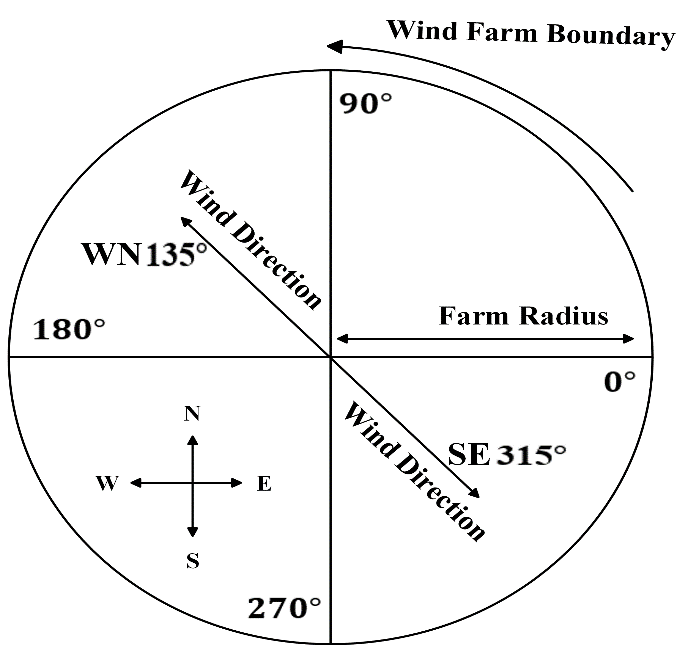
\includegraphics[scale=0.6]{wind farm.png}
\caption{A circular wind farm}
\label{fig:wind farm}
\end{figure}

    \item \textbf{WFLOP Mathematical Model:}
    The mathematical model of WFLOP contains two parts: the wake effect model and the power output model. The wake effect model captures the reduction in power generation experienced by downstream turbines due to the wake induced by upstream turbines. Jensen's wake model~\cite{Jensen1983, Katic1986} is a widely used model for solving WFLOP. The power output model used in WFLOP is considered from Kusiak and Song~\cite{Kusiak2010}.

    \item \textbf{Objective:}
    This study aims to maximize the power generation by minimizing wake-induced losses, while satisfying two constraints obtained from assumptions (6) and (8).

\end{enumerate}

\subsection{\textbf{The Wake Effect Model}}

The wake effect can lead to a substantial reduction in the wind speed experienced by downstream turbines as a result of momentum extraction and wake expansion. Therefore, accounting for wake losses is a critical aspect of wind farm layout design. Jensen's wake model~\cite{Jensen1983,Katic1986} is retained here because it is computationally inexpensive and has been used extensively in the legacy WFLOP benchmark literature against which the present results are compared. This choice is made for \emph{benchmark comparability}, not because Jensen is the most accurate contemporary wake model. Gaussian and three-dimensional wake formulations can represent the velocity field more realistically and have been used successfully in WFLO studies~\cite{Tao2020,Cao2022}; consequently, the numerical conclusions below are model-dependent.

When a uniform wind comes into contact with a turbine, it creates turbulence, and a wake expands linearly downstream, causing a reduction in wind speed, i.e., from upstream wind speed $s_{\text{up}}$ to downstream wind speed $s_{\text{down}}$. Figure~\ref{fig:wake-model} illustrates the wake model of WFLOP.

\begin{figure}[htbp]
\centering
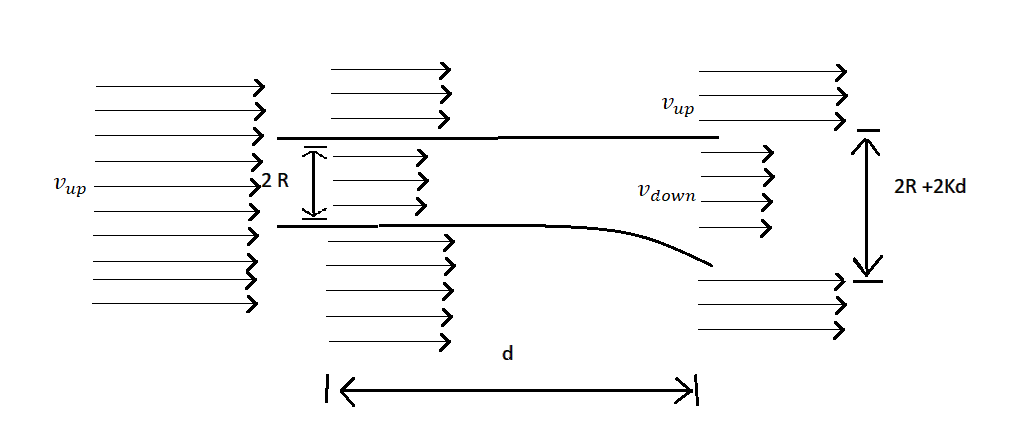
\includegraphics[scale=0.5]{wake mode.png}
\caption{Wake model representation for wind turbine layout}
\label{fig:wake-model}
\end{figure}

Let $s_{\text{up}}$ represent the wind speed before encountering the turbine, $s_{\text{down}}$ represent the downstream wind speed, $K$ be the wake spreading constant, $d$ be the inter-turbine distance, and $R$ be the rotor radius of the turbine.

The velocity deficit induced at turbine $j$ resulting from the wake generated by turbine $i$ is given by:
\begin{align*}
    \delta s_{ij} = 1-(s_{\text{down}}/s_{\text{up}})=\frac{1 - \sqrt{1 - C_T}}{\left(1 + \frac{K d_{ij}}{R}\right)^2}
\end{align*}

where $C_T$ denotes the turbine thrust coefficient, and $d_{ij}$ represents the inter-turbine distance between turbines $i$ and $j$.

If a turbine is influenced by the wakes of multiple upstream turbines, the total velocity deficit for that turbine is the superposition of the velocity deficits due to each wake. Assuming turbine $i$ is influenced by the wakes of $N$ turbines, then the overall deficit can be computed as follows:

\begin{align}\label{eq:veldeficit2}
    \delta s_i = \sqrt{ \sum_{\substack{j=1 \\ j \ne i}}^{N} (\delta s_{ij})^2}.
\end{align}

Each turbine rotor is positioned perpendicular to the prevailing wind direction $\theta$ to ensure maximum energy capture. When wind passes downstream of a turbine located at $(\rho, \sigma)$, the resulting wake can be idealized as an imaginary half cone. Figure~\ref{fig:half-cone} indicates this half cone generated by a turbine positioned at $(\rho, \sigma)$.

\begin{figure}[htbp]
\centering
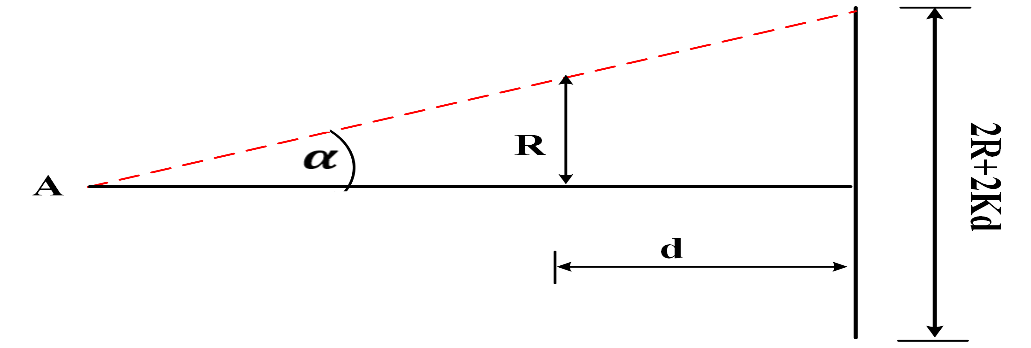
\includegraphics[width=0.7\linewidth]{half cone.png}
\caption{Geometric representation of the wake expansion angle $\alpha$}
\label{fig:half-cone}
\end{figure}

\noindent where $A$ is the imaginary vertex of the half cone representing the wake region. The geometry of the cone is governed by the wake spreading constant $K$, $\alpha$ ($0 \leq \alpha \leq \pi/2$) is the half-cone angle, i.e., the angle between the central axis and the side of the cone. The value of $\alpha$ is computed as $\alpha = \arctan(K)$. This imaginary half cone is used to model the influence of wake effects from one turbine on others within the wind farm.


\textbf{Lemma 1.} For a specified wind direction \( \theta \), the angle \( \beta_{ij} \), where \( 0 \leq \beta_{ij} \leq \pi \), represents the angle between the two vectors extending from point \( A \) to turbines \( i \) and \( j \) and it can be computed using the following expression:

\[
\beta_{ij} = \cos^{-1}\!\left(\frac{u_{ij}}{\sqrt{u_{ij}^2+v_{ij}^2}}\right),
\]
with
\begin{align*}
u_{ij}&=(\rho_i - \rho_j)\cos\theta + (\sigma_i - \sigma_j)\sin\theta + \tfrac{R}{K},\\
v_{ij}&=-(\rho_i - \rho_j)\sin\theta + (\sigma_i - \sigma_j)\cos\theta ,
\end{align*}

\noindent
where \( \frac{R}{K} \) denotes the distance from the rotor center to the virtual vertex \( A \) of the wake cone.

\textbf{Lemma 2.} If turbine \( i \) is positioned within the wake generated by turbine \( j \), the distance between these, along the wind direction \( \theta \) is given by:

\begin{align*}
d_{ij} = \left| (\rho_i - \rho_j)\cos\theta + (\sigma_i - \sigma_j)\sin\theta \right|.
\end{align*}

The equation \eqref{eq:veldeficit2} is then expressed by restricting the summation to those turbines \( j \) where \( j \neq i \) and \( \beta_{ij} < \alpha \):

\begin{align}\label{eq5}
\delta s_i = \sqrt{ \sum_{\substack{j = 1 \\ j \ne i,\, \beta_{ij} < \alpha}}^{N} \left( \delta s_{ij} \right)^2 }.
\end{align}

\noindent
Equation \eqref{eq5} indicates that \( \delta s_i\) is a function of both the wind direction \( \theta \) and the turbine \( i \)'s location (i.e., \( (\rho_i, \sigma_i) \)).

\medskip

\noindent
The transformation of the Weibull parameter is made explicit as follows. For a fixed directional bin $\theta$, let the free-stream speed be
\[
S_\theta \sim \mathrm{Weibull}\!\left(\zeta(\theta),\psi(\theta)\right).
\]
Under the present Jensen benchmark, the combined deficit $\delta s_i(\theta)$ is treated as a deterministic multiplicative reduction within that directional bin, so the local inflow at turbine $i$ is
\[
S_{i,\theta}=\left[1-\delta s_i(\theta)\right]S_\theta .
\]
For a positive constant $a$, if $S\sim\mathrm{Weibull}(\zeta,\psi)$, then $aS\sim\mathrm{Weibull}(\zeta,a\psi)$. Hence the shape parameter is unchanged while the scale parameter becomes
\begin{align}
\psi_i(\theta) &= \psi(\theta)\left[1-\delta s_i(\theta)\right],
\quad i=1,2,\ldots,N. \label{eq:weibull-scale}
\end{align}
This scaling is physically consistent with the \emph{specific simplifying assumption} that the wake model acts as a deterministic speed multiplier for a given direction bin. It should not be interpreted as a general turbulence model; more detailed wake/turbulence models may alter the full wind-speed distribution rather than only its scale.

\subsection{The Power Model}
\label{sec:powermodel}

The power model follows the simplified Kusiak--Song benchmark used by the comparison studies~\cite{Kusiak2010}. It is a computational surrogate for a manufacturer power curve rather than a claim of high-fidelity turbine aerodynamics:
\begin{align}\label{eq7}
f(s) =
\begin{cases}
0, & s < s_{\text{cut-in}},\\
\lambda' s + \eta, & s_{\text{cut-in}} \leq s \leq s_{\text{rated}},\\
P_{\text{rated}}, & s > s_{\text{rated}}.
\end{cases}
\end{align}
Here $s_{\text{cut-in}}$ and $s_{\text{rated}}$ are the benchmark cut-in and rated speeds, while $\lambda'$ and $\eta$ define the linear segment. The legacy benchmark does not explicitly model a cut-out shutdown in the subsequent analytical integral; the present manuscript therefore uses the model consistently as written above. This simplification improves comparability with prior WFLOP results but can introduce error relative to a turbine-specific nonlinear power curve. Rather than assuming this error is negligible, Section~\ref{sec:powercurve} re-evaluates the stored layouts with a nonlinear (cubic) power curve, with and without a 25~m/s cut-out, and reports the resulting change in expected power and in the algorithm ordering.

For a turbine positioned at \( (\rho, \sigma) \) and wind direction \( \theta \), the expected power output is given by:

\begin{multline}\label{eq8}
E(P_i) = \int_0^{360} P_\theta(\theta) \cdot E(P_i,\theta) \, d\theta \\= \int_0^{360} P_\theta(\theta) \cdot \int_0^{\infty} f(s) \cdot
       p_s(s, \zeta(\theta), \psi_i(\theta)) \, ds \, d\theta .
\end{multline}

Thus, the optimization problem is formulated with the objective of maximizing the total power output of the wind farm, subject to the spatial and operational constraints defined by assumptions (6) and (8). The mathematical formulation is:

\begin{align*}
\text{Maximize} \quad & \sum_{i=1}^{N} E(P_i) \notag \\
\text{subject to} \quad & (\rho_i - \rho_j)^2 + (\sigma_i - \sigma_j)^2 \geq 64R^2, \notag \\
& \rho_i^2 + \sigma_i^2 \leq r^2, \quad i,j=1,2,\dots,N,\ i \neq j
\end{align*}

where $\text{E}(P_i)$ corresponds to the expected power output of the $i^\text{th}$ turbine under the adopted benchmark model. The piecewise-linear representation in \eqref{eq7} is retained for consistency with the historical comparison, not because its approximation error is assumed negligible. Incorporating Equation~\eqref{eq7} and the Weibull model, Equation~\eqref{eq8} becomes:

\begin{align*}
&E(P_i) = \int_0^{360} p_\theta(\theta) \int_0^{\infty} f(s) p_s(s, \zeta(\theta), \psi_i(\theta)) \, ds \, d\theta \notag \\
&= \int_0^{360} p_\theta(\theta) \int_0^{\infty}  \frac{f(s)\zeta(\theta)}{\psi_i(\theta)} \left[\frac{s}{\psi_i(\theta)}\right]^{\zeta(\theta)-1} e^{-\left[\frac{s}{\psi_i(\theta)}\right]^{\zeta(\theta)}} ds \, d\theta \notag \\
&= \int_0^{360} p_\theta(\theta) \Bigg[ \lambda' \int_{s_{\text{cut-in}}}^{s_{\text{rated}}}   \frac{s\zeta(\theta)}{\psi_i(\theta)}\left[\frac{s}{\psi_i(\theta)}\right]^{\zeta(\theta)-1} e^{-\left[\frac{s}{\psi_i(\theta)}\right]^{\zeta(\theta)}} ds \notag \\
&\quad + \eta \int_{s_{\text{cut-in}}}^{s_{\text{rated}}} \frac{\zeta(\theta)}{\psi_i(\theta)} \left(\frac{s}{\psi_i(\theta)}\right)^{\zeta(\theta)-1} e^{-\left(\frac{s}{\psi_i(\theta)}\right)^{\zeta(\theta)}} ds \notag \\
&\quad + P_{\text{rated}} \int_{s_{\text{rated}}}^{\infty} \frac{\zeta(\theta)}{\psi_i(\theta)} \left(\frac{s}{\psi_i(\theta)}\right)^{\zeta(\theta)-1} e^{-\left(\frac{s}{\psi_i(\theta)}\right)^{\zeta(\theta)}} ds \Bigg].
\end{align*}

Wind direction and speed are discretized into $N_\theta + 1$ and $N_s + 1$ bins, respectively, using equal bin widths to approximate the integration part using the Riemann sum~\cite{Stroock1999}. The discretization approach for estimating expected power output was described by Kusiak and Song~\cite{Kusiak2010}.

Let wind direction bins be defined by $\theta_0 = 0^\circ, \theta_1, \ldots, \theta_{N_\theta+1} = 360^\circ$ and wind speed bins between $s_{\text{cut-in}}$ and $s_{\text{rated}}$ be $s_0 = s_{\text{cut-in}}, s_1, \ldots, s_{N_s+1} = s_{\text{rated}}$.

Using the Riemann sum approximation~\cite{Stroock1999}, the expected power output of the \( i^{\text{th}} \) turbine is estimated as:
\begin{align*}
&E(P_i) = \lambda' \sum_{j=1}^{N_s+1} \left(\frac{s_{j-1} + s_j}{2}\right) \sum_{l=1}^{N_\theta+1} (\theta_l - \theta_{l-1}) \omega_{l-1}  \notag \\
&\Bigg[ e^{-\left(\frac{s_{j-1}}{\psi_i\left(\frac{\theta_l + \theta_{l-1}}{2}\right)}\right)^{\zeta\left(\frac{\theta_l + \theta_{l-1}}{2}\right)}}- e^{-\left(\frac{s_j}{\psi_i\left(\frac{\theta_l + \theta_{l-1}}{2}\right)}\right)^{\zeta\left(\frac{\theta_l + \theta_{l-1}}{2}\right)}} \Bigg]  \notag \\
&+P_{\text{rated}} \sum_{l=1}^{N_\theta+1} (\theta_l - \theta_{l-1}) \omega_{l-1} e^{-\left(\frac{s_{\text{rated}}}{\psi_i\left(\frac{\theta_l + \theta_{l-1}}{2}\right)}\right)^{\zeta\left(\frac{\theta_l + \theta_{l-1}}{2}\right)}} \\
& + \eta \sum_{l=1}^{N_\theta+1} (\theta_l - \theta_{l-1}) \omega_{l-1} \\
&\Bigg[ e^{-\left(\frac{s_{\text{cut-in}}}{\psi_i\left(\frac{\theta_l + \theta_{l-1}}{2}\right)}\right)^{\zeta\left(\frac{\theta_l + \theta_{l-1}}{2}\right)}} - e^{-\left(\frac{s_{\text{rated}}}{\psi_i\left(\frac{\theta_l + \theta_{l-1}}{2}\right)}\right)^{\zeta\left(\frac{\theta_l + \theta_{l-1}}{2}\right)}} \Bigg].
\end{align*}

Here, $N_s$ and $N_\theta$ denote the count of intervals for wind speed and wind direction, respectively, and $\omega_{l-1}$ is the wind blowing probability for the $(l-1)$-th wind direction bin.

\paragraph{Interpretation of the reported benchmark objective.}
The numerical tables retain the historical discretization convention of the adopted WFLOP benchmark, including the directional-bin-width factor $(\theta_l-\theta_{l-1})$. The resulting tabulated ``power'' values are therefore best interpreted as \emph{benchmark objective values under that legacy convention} for comparison with prior studies, rather than as instantaneous electrical power that must be bounded by $N P_{\text{rated}}$. Because all 24 bins have the same width of $15^\circ$ and $\sum_l\omega_{l-1}=1$, the reported objective equals $15$ times the expected farm power in kW. For example, the free-stream (ideal) objective of a single turbine is $14045.74$ for Wind Data Set~I, which corresponds to an expected power of $936.38$~kW, i.e., a capacity factor of $0.624$ and an annual energy production (AEP) of $936.38\times8.76=8202.7$~MWh. In general, $\mathrm{AEP}\,[\mathrm{MWh}] = (\text{objective}/15)\times 8.76$. This conversion was confirmed with the independent evaluator described in Section~\ref{sec:validation}. This distinction is important when comparing the benchmark numbers with physical nameplate capacity.


\subsection{Constraint Handling Mechanism}
\label{sec:constraints}

The WFLOP search must satisfy the circular farm boundary and the minimum inter-turbine spacing. The implementation used for all reported runs handles both constraints with two explicit operations: a box repair of the decision variables and a large additive penalty in the minimized objective. No other repair or displacement operator is applied.

\subsubsection{Box Repair}
Every coordinate of every candidate is clipped to the bounding square of the farm after each position update,
\begin{align*}
\rho_i&\leftarrow\min\{\max\{\rho_i,-r\},r\},\\
\sigma_i&\leftarrow\min\{\max\{\sigma_i,-r\},r\}.
\end{align*}
This guarantees bounded decision variables but not the circular constraint $\rho_i^2+\sigma_i^2\le r^2$, which is enforced through the penalty below.

\subsubsection{Violation Measure}
The benchmark constraints are $d_{ij}=\sqrt{(\rho_i-\rho_j)^2+(\sigma_i-\sigma_j)^2}\ge d_{\min}=8R$ for all $i\ne j$ and $\sqrt{\rho_i^2+\sigma_i^2}\le r$ for all $i$. Their aggregate violation is
\begin{equation}
V=\sum_{i<j}\max\{0,\,d_{\min}-d_{ij}\}+\sum_{i=1}^{N}\max\Bigl\{0,\,\sqrt{\rho_i^2+\sigma_i^2}-r\Bigr\},
\label{eq:spacingviolation}
\end{equation}
and a layout is feasible if and only if $V=0$.

\subsubsection{Penalized Objective}
All optimizers minimize the penalized wake loss
\begin{equation}
F_p=\Bigl(N E_{\rm ideal}-\sum_{i=1}^{N}E(P_i)\Bigr)+\lambda V,\qquad \lambda=10^{10},
\label{eq:penalty}
\end{equation}
where $N E_{\rm ideal}$ is the wake-free value of the objective, so the first term is the wake loss reported in the tables. Because $\lambda$ exceeds any attainable wake loss by many orders of magnitude, comparing $F_p$ values implements feasibility-first selection:
\begin{itemize}
\item any feasible candidate is preferred to an infeasible one;
\item between two feasible candidates, the one with the smaller wake loss (larger objective) is preferred;
\item between two infeasible candidates, the one with the smaller total violation $V$ is preferred.
\end{itemize}
Box repair is applied after every position update and $F_p$ is used in every comparison, sort and greedy selection of Algorithms~\ref{alg:lx-ssa} and~\ref{alg:lx-ssa-wflop}. The same objective, including the penalty, is used for SSA, LX-SSA, PSO and DE. Section~\ref{sec:equalbudget} shows that a radial projection onto the circle, used instead of box clipping, changes the attained objective values, so the boundary-handling rule is part of the experimental protocol.

\section{\textbf{Previously Developed Laplacian Salp Swarm Algorithm (LX-SSA)}}

LX-SSA was introduced by Solanki and Deep in 2023~\cite{Solanki2023}; the algorithmic novelty belongs to that publication. The present paper only summarizes the operators needed to understand and reproduce the WFLOP application. Consistent with the published SSA/LX-SSA implementation, the sorted population is divided into a leader subgroup (first half) and a follower subgroup (second half), while the best solution found so far is retained as the food source $H$~\cite{Mirjalili2017,Solanki2023}. LX-SSA keeps these SSA dynamics and supplements the follower update with a Laplace-based candidate and greedy retention~\cite{Solanki2023,Deep2007}.

For a leader salp $i\le N_p/2$, the $j$th coordinate is updated around the food source as
\begin{align}\label{eq12}
\rho_j^i =
\begin{cases}
H_j+r_1\big((ub_j-lb_j)r_2+lb_j\big), & r_3\ge0.5,\\
H_j-r_1\big((ub_j-lb_j)r_2+lb_j\big), & r_3<0.5,
\end{cases}
\end{align}
where $r_2,r_3\sim U(0,1)$ and
\[
r_1=2\exp\!\left[-\left(\frac{4l}{L}\right)^2\right],
\]
with iteration $l$ and maximum iteration $L$. For follower salps $i>N_p/2$, the standard SSA position is formed from the current and preceding salps:
\begin{align}\label{eq14}
\rho_j^i=\frac{1}{2}\left(\rho_j^i+\rho_j^{i-1}\right).
\end{align}

LX-SSA then forms an additional follower candidate
\begin{align}\label{eq15}
y_j^i=x_j^i+\gamma(z,\phi,\chi)\left(H_j-x_j^i\right),
\end{align}
where $x_j^i$ is the current follower coordinate and
\begin{align}\label{eq16}
\gamma(z,\phi,\chi)=
\begin{cases}
\phi+\chi\ln(2z), & z\le0.5,\\
\phi-\chi\ln\bigl(2(1-z)\bigr), & z>0.5,
\end{cases}
\end{align}
with $z\sim U(0,1)$, which is the inverse-distribution-function sample of a Laplace variable with location $\phi$ and scale $\chi$ (mean $\phi$, variance $2\chi^2$). The location parameter $\phi$ centers the Laplace variate, whereas the scale parameter $\chi>0$ controls its dispersion and therefore the perturbation magnitude. Smaller $\chi$ concentrates moves near the center; larger $\chi$ increases the probability of longer exploratory moves. All experiments use $\phi=0$ and $\chi=1$, so that $\gamma$ is symmetric about zero with $P(|\gamma|>1)=e^{-1}\approx0.37$: most follower candidates move towards $H$ ($\gamma>0$) or away from it ($\gamma<0$) by a fraction of the current distance, while a heavy tail occasionally produces moves beyond $H$ or well away from it. These values are fixed for every WFLOP case and are not tuned to WFLOP; no WFLOP-specific sensitivity analysis of $\phi$ and $\chi$ was carried out. Because each follower evaluates both candidates before the population is re-evaluated, one LX-SSA iteration costs $N_p/2\times2+N_p=2N_p$ objective calls, twice the $N_p$ calls of an SSA iteration; comparisons at equal numbers of calls are therefore reported in Section~\ref{sec:equalbudget}.

Algorithm~\ref{alg:lx-ssa} follows the published leader/follower logic and avoids the earlier ambiguity in which a follower update appeared inside the leader branch. It also avoids hard-coding a minimization inequality; ``better'' is determined by the objective sense and, for WFLOP, by the feasibility rules in Section~\ref{sec:constraints}.

\begin{algorithm}
\caption{Previously developed LX-SSA search logic~\cite{Solanki2023}}
\label{alg:lx-ssa}
\begin{algorithmic}[1]
\State Initialize and evaluate the salp population; sort it and set the best solution as food source $H$.
\While{the termination criterion is not met}
    \State Update $r_1$.
    \For{salp $i=1,\ldots,N_p$}
        \If{$i\le N_p/2$}
            \State Update leader $i$ using \eqref{eq12}.
        \Else
            \State Form the standard follower candidate using \eqref{eq14}.
            \State Draw $\gamma(z,\phi,\chi)$ using \eqref{eq16}.
            \State Form the Laplace-based follower candidate using \eqref{eq15}.
            \State Evaluate both follower candidates and retain the better one.
        \EndIf
    \EndFor
    \State Enforce variable bounds, re-evaluate the population, sort, and update $H$.
\EndWhile
\State \Return the best solution $H$.
\end{algorithmic}
\end{algorithm}

The comparison between SSA and LX-SSA in the WFLOP experiments can therefore be interpreted as a practical mechanism-level comparison of the baseline SSA dynamics against the additional Laplace-based follower candidate. The original historical-table sample vectors are not retained in that archive. Separate run-level DS1/DS2 workbooks support the explicitly labelled follow-up analysis in Section~\ref{sec:additional-runlevel}; their samples are not substituted for the original tabulated results.

\section{\textbf{Application of LX-SSA to the Wind Farm Layout Optimization Problem (WFLOP)}}

The published LX-SSA~\cite{Solanki2023} is employed without algorithmic redesign. For a prescribed number $N$ of turbines, candidate $j$ is represented by
\[
\mathbf{x}_j=(\rho_j^1,\sigma_j^1,\rho_j^2,\sigma_j^2,\ldots,\rho_j^N,\sigma_j^N)\in\mathbb{R}^{2N}.
\]
The optimizer therefore searches only the turbine coordinates; $N$ is fixed during a run. The objective and constraint calculations are the WFLOP model described above.

Algorithm~\ref{alg:lx-ssa-wflop} makes the implementation sequence explicit. In particular, the candidate coordinates are updated first, box repair is applied, wake deficits and Weibull-scale adjustments are recomputed, the constraint violation is measured, and all comparisons use the penalized objective $F_p$, which implements feasibility-first selection (Section~\ref{sec:constraints}). This ordering is essential because the objective depends on the layout-dependent wake field.

\begin{algorithm}
\caption{Application of LX-SSA to WFLOP for a prescribed turbine count $N$}
\label{alg:lx-ssa-wflop}
\begin{algorithmic}[1]
\Require Farm radius $r$, prescribed $N$, wind data, turbine/wake parameters, population size $N_p$, maximum iterations $T$, $\phi$, $\chi$
\State Set dimension $d=2N$, bounds $[-r,r]^d$, and draw $N_p$ coordinate vectors uniformly in the bounds.
\For{each candidate}
    \State For each wind-direction bin, compute wake deficits $\delta s_i(\theta)$.
    \State Set $\psi_i(\theta)$ using \eqref{eq:weibull-scale} and compute $E(P_i)$.
    \State Compute $V$ from \eqref{eq:spacingviolation} and the penalized objective $F_p$ from \eqref{eq:penalty}.
\EndFor
\State Sort the population by $F_p$ and set the best candidate as food source $H$.
\For{$t=1$ to $T$}
    \State Generate the leader and follower candidates of Algorithm~\ref{alg:lx-ssa}, applying box repair to each; followers keep the better of their two candidates by $F_p$.
    \State Apply box repair, evaluate $F_p$ for the new population and sort it.
    \State If the best new candidate has a smaller $F_p$ than $H$, replace $H$.
\EndFor
\State \Return $H$ and its turbine coordinates, objective value, wake loss and feasibility status.
\end{algorithmic}
\end{algorithm}

No claim is made that this mapping changes the mathematical definition of LX-SSA. Its contribution is the explicit integration of the existing optimizer with the continuous WFLOP representation and constraints.

\begin{table*}[htbp]
\centering
\caption{Wind Data Sets I and II: Direction Intervals, Weibull Parameters, and Blowing Probabilities}
\begin{minipage}{0.49\textwidth}
\centering
\begin{tabular}{cccccc}
\toprule
\textbf{Int.} & \textbf{Start ($^\circ$)} & \textbf{End ($^\circ$)} & \textbf{$\zeta$}  & \textbf{$\psi$} & \textbf{Prob.} \\
\midrule
1  & 0   & 15  & 2 & 13   & 0.000 \\
2  & 15  & 30  & 2 & 13   & 0.010 \\
3  & 30  & 45  & 2 & 13   & 0.010 \\
4  & 45  & 60  & 2 & 13   & 0.010 \\
5  & 60  & 75  & 2 & 13   & 0.010 \\
6  & 75  & 90  & 2 & 13   & 0.200 \\
7  & 90  & 105 & 2 & 13   & 0.600 \\
8  & 105 & 120 & 2 & 13   & 0.010 \\
9  & 120 & 135 & 2 & 13   & 0.010 \\
10 & 135 & 150 & 2 & 13   & 0.010 \\
11 & 150 & 165 & 2 & 13   & 0.010 \\
12 & 165 & 180 & 2 & 13   & 0.010 \\
13 & 180 & 195 & 2 & 13   & 0.010 \\
14 & 195 & 210 & 2 & 13   & 0.010 \\
15 & 210 & 225 & 2 & 13   & 0.010 \\
16 & 225 & 240 & 2 & 13   & 0.010 \\
17 & 240 & 255 & 2 & 13   & 0.010 \\
18 & 255 & 270 & 2 & 13   & 0.010 \\
19 & 270 & 285 & 2 & 13   & 0.010 \\
20 & 285 & 300 & 2 & 13   & 0.010 \\
21 & 300 & 315 & 2 & 13   & 0.010 \\
22 & 315 & 330 & 2 & 13   & 0.010 \\
23 & 330 & 345 & 2 & 13   & 0.010 \\
24 & 345 & 360 & 2 & 13   & 0.000 \\
\bottomrule
\end{tabular}
\label{tab:wind_data_I}
\end{minipage}
\hfill
\begin{minipage}{0.49\textwidth}
\centering
\begin{tabular}{cccccc}
\toprule
\textbf{Int.} & \textbf{Start ($^\circ$)} & \textbf{End ($^\circ$)} & \textbf{$\zeta$} & \textbf{$\psi$} & \textbf{Prob.} \\
\midrule
1  & 0   & 15  & 2 & 7.0  & 0.0002 \\
2  & 15  & 30  & 2 & 5.0  & 0.0080 \\
3  & 30  & 45  & 2 & 5.0  & 0.0227 \\
4  & 45  & 60  & 2 & 5.0  & 0.0242 \\
5  & 60  & 75  & 2 & 5.0  & 0.0225 \\
6  & 75  & 90  & 2 & 4.0  & 0.0339 \\
7  & 90  & 105 & 2 & 5.0  & 0.0423 \\
8  & 105 & 120 & 2 & 6.0  & 0.0290 \\
9  & 120 & 135 & 2 & 7.0  & 0.0617 \\
10 & 135 & 150 & 2 & 7.0  & 0.0813 \\
11 & 150 & 165 & 2 & 8.0  & 0.0994 \\
12 & 165 & 180 & 2 & 9.5  & 0.1394 \\
13 & 180 & 195 & 2 & 10.0 & 0.1839 \\
14 & 195 & 210 & 2 & 8.5  & 0.1115 \\
15 & 210 & 225 & 2 & 8.5  & 0.0765 \\
16 & 225 & 240 & 2 & 6.5  & 0.0080 \\
17 & 240 & 255 & 2 & 4.6  & 0.0051 \\
18 & 255 & 270 & 2 & 2.6  & 0.0019 \\
19 & 270 & 285 & 2 & 8.0  & 0.0012 \\
20 & 285 & 300 & 2 & 5.0  & 0.0010 \\
21 & 300 & 315 & 2 & 6.4  & 0.0017 \\
22 & 315 & 330 & 2 & 5.2  & 0.0031 \\
23 & 330 & 345 & 2 & 4.5  & 0.0097 \\
24 & 345 & 360 & 2 & 3.9  & 0.0317 \\
\bottomrule
\end{tabular}
\label{tab:wind_data_II}
\end{minipage}
\end{table*}


\section{\textbf{Experimental Analysis}}
\subsection{\textbf{Experimental Setup and Wind Data Sets}}

In this study, two distinct wind data sets, referred to as \textit{Wind Data Set I} and \textit{Wind Data Set II}, are employed to evaluate the performance of LX-SSA on WFLOP. The characteristics of these data sets are summarized in Table~\ref{tab:wind_data_I} (left: Data Set~I; right: Data Set~II). For both data sets, the wind direction range is discretized into 24 bins, with each bin representing a $15^\circ$ directional interval, providing a detailed distribution of wind patterns across different directions.

Table~\ref{tab:wind_data_I} summarizes the key Weibull distribution parameters including shape parameter $(\zeta)$, scale parameter $(\psi)$ and the wind blowing probability $(\omega_{l-1})$ for each wind direction interval ranging from $\theta_{l-1}$ to $\theta_l$.

LX-SSA and SSA are employed on both wind data sets to solve WFLOP across three wind-farm radii: 500~m, 750~m, and 1000~m. The turbine count is \emph{fixed a priori within each optimization run}; separate cases are solved for different prescribed values of $N$ (from 2 up to 15, depending on farm radius). Consequently, the present study optimizes turbine coordinates for a given $N$ and does not claim simultaneous optimization of turbine number and turbine locations. The result tables also include QA-SSA~\cite{SolankiQA2024} values available in the experiment archive. EA, ACO, PF, and BBO columns are retained as historical benchmark values reported by earlier WFLOP studies and are not treated as if they had been re-run under the present code, seeds, or hardware.

Section~\ref{sec:experimental-results} presents and analyzes the results obtained from solving WFLOP using both LX-SSA and SSA.

To assess the effectiveness of LX-SSA, the following experimental framework is employed:

\begin{itemize}
    \item Population size, $N_p = 5 \times$ (count of decision variables)
    \item Maximum generations/iterations: 100
    \item Total independent runs: 30
    \item Rotor radius, $R = 38.5$ m
    \item Cut-in wind speed, $s_{\text{cut-in}} = 3.5$ m/s
    \item Rated wind speed, $s_{\text{rated}} = 14$ m/s
    \item Rated power output, $P_{\text{rated}} = 1500$ kW
    \item Linear model parameters: $\lambda' = 140.86$, $\eta = -500$
    \item Thrust coefficient, $c_T = 0.8$
    \item Wake spreading constant, $K = 0.075$
    \item LX-SSA Laplace parameters: $\phi=0$, $\chi=1$; constraint penalty $\lambda=10^{10}$
\end{itemize}

The follow-up and controlled experiments (Sections~\ref{sec:additional-runlevel} and~\ref{sec:equalbudget}) use a population of 30 for all algorithms, PSO with inertia weight $w=0.7$ and acceleration coefficients $c_1=c_2=2$ (velocities unbounded, positions clipped to the bounds), and DE/rand/1/bin with $F=0.5$ and $CR=0.9$. All algorithms draw their initial population uniformly in $[-r,r]^{2N}$ and use the same penalized objective~\eqref{eq:penalty}.

The minimum spacing is $4D=8R=308$~m under the benchmark convention. All stochastic summary values in the tables are based on the archived 30-run summaries. The original six result tables lack their individual run-level vectors, seeds and wall-clock logs. A distinct DS1/DS2 follow-up archive does contain labelled seeds, individual solutions, coordinates and aggregate per-case wall-clock times; the optimizer settings listed above were taken from the implementation, whereas the hardware/software configuration of the archived runs is not recorded. The controlled re-runs of Section~\ref{sec:equalbudget} were therefore timed on a documented machine. To support reproducibility within these limits, the revision supplies the stored follow-up run records with final coordinates, the best-layout coordinates of the selected cases (Appendix~\ref{app:coordinates}), and an independent evaluator that reproduces the recorded objective values (Section~\ref{sec:validation}).

In this study, wind speed is categorized into $N_s = 20$ intervals, each with a width of 0.5 m/s, starting from cut-in wind speed $s_{\text{cut-in}}$ up to rated wind speed $s_{\text{rated}}$. Similarly, wind direction is categorized into $N_{\theta} = 24$ intervals, each covering $15^{\circ}$, encompassing a total of $360^{\circ}$.

\subsection*{Wind Data Set I}
Wind Data Set I, described in Table~\ref{tab:wind_data_I}, assumes fixed Weibull parameters ($\zeta=2$, $\psi=13$) for all wind direction intervals. However, the blowing probability $\omega_l$ varies by direction. Notably, $\omega_0 = \omega_{23} = 0$ implies no wind in the first and last intervals. The wind blowing probabilities in the 6th and 7th intervals are $\omega_5 = 0.2$ and $\omega_6 = 0.6$, respectively. For all other intervals, $\omega_l = 0.01$ for $l \notin \{0, 5, 6, 23\}$.

\subsection*{Wind Data Set II}
As presented in the right half of Table~\ref{tab:wind_data_I}, this data set maintains a constant shape parameter $\zeta = 2$, but allows the scale parameter $\psi$ to vary across wind direction intervals. The interval from $255^{\circ}$ to $270^{\circ}$ exhibits the smallest scale parameter $\psi = 2.6$, while intervals from $165^{\circ}$ to $180^{\circ}$ and $180^{\circ}$ to $195^{\circ}$ possess the highest value $\psi = 10$.


%\section{\textbf{Experimental Results}}
%\label{sec:experimental-results}

\subsection{\textbf{Performance Analysis}}
\label{sec:experimental-results}
For each prescribed turbine count, the optimizer searches for turbine coordinates that maximize the adopted benchmark objective subject to the stated boundary and spacing constraints. The sequence of cases with different $N$ is a parameter sweep; it does not identify an ``optimal turbine count'' unless an explicit cost/capacity objective is added. The following results compare LX-SSA with the classical SSA mechanism-level baseline for farm radii of 500, 750, and 1000~m, while the remaining historical columns provide contextual benchmark values. The individual runs underlying the original six tables are unavailable, so those specific table differences remain descriptive. A separate analysis of newly supplied DS1/DS2 run vectors is reported in Section~\ref{sec:additional-runlevel}.


\paragraph{\textbf{Wind farm radius 500~m:}}
Tables~\ref{tab:500mI} and~\ref{tab:500mII} report the available benchmark objective and wake-loss values for Wind Data Sets I and II. The historical ACO, PF and BBO studies cited in the table context considered smaller turbine-count ranges, whereas the present archive contains prescribed LX-SSA/SSA cases through $N=10$. This difference in the tested range should not be interpreted as proof that one algorithm has discovered a larger physical ``capacity'' of the farm, because $N$ is fixed before each optimization run. For common prescribed values of $N$, LX-SSA can be compared directly with SSA on the same WFLOP formulation. The corresponding archived layouts are shown in Figs.~\ref{fig:layout500I} and~\ref{fig:layout500II}.

\paragraph{\textbf{Wind farm radius 750~m:}}
Tables~\ref{tab:750mI} and~\ref{tab:750mII} contain the 750~m results for prescribed turbine counts through $N=12$. Within the archived SSA/LX-SSA comparisons, the LX-SSA entries are generally at least as high in the benchmark objective and often lower in wake loss, but the magnitude of the objective difference is small. These historical-table observations remain descriptive because their corresponding individual run records have not been supplied. The archived layouts are shown in Figs.~\ref{fig:layout750I} and~\ref{fig:layout750II}.

\paragraph{\textbf{Wind farm radius 1000~m:}}
Tables~\ref{tab:1000mI} and~\ref{tab:1000mII} report the largest benchmark cases considered here, with prescribed turbine counts through $N=15$. LX-SSA remains numerically competitive with SSA in these cases, with the same caution that ``15 turbines'' is only the largest value tested and is not a universal feasibility limit for a 1000~m circular farm. Since the largest case still contains only 15 turbines, the present evidence should not be interpreted as a large-scale scalability demonstration. The archived layouts are shown in Figs.~\ref{fig:layout1000I} and~\ref{fig:layout1000II}.

\subsection{Interpretation of the SSA--LX-SSA Comparison}
SSA is the most informative ablation-style baseline available in the present archive because LX-SSA inherits the SSA framework and adds the Laplace-based candidate mechanism. Thus, comparing SSA and LX-SSA under the same WFLOP formulation provides evidence about the practical effect of that additional mechanism on this application. The tabulated differences in the benchmark power objective are generally small in relative terms, while wake-loss differences are more visible in a number of cases. The manuscript therefore avoids phrases such as ``significantly outperforms'' unless a formal test is supported by run-level data. The equal-budget re-runs of Section~\ref{sec:equalbudget} provide this mechanism-level test directly and show no equal-cost advantage of LX-SSA over SSA.

QA-SSA~\cite{SolankiQA2024} is retained as an additional SSA-family comparator where values are available. EA, ACO, PF, and BBO entries are literature benchmarks and should not be interpreted as a controlled head-to-head experiment. PSO/DE run-level comparisons are reported in Section~\ref{sec:additional-runlevel} (recorded, unequal budgets) and Section~\ref{sec:equalbudget} (controlled, equal budgets). VNS, gradient/pseudo-gradient approaches, and surrogate/data-driven methods remain important baselines for future benchmarking~\cite{Cazzaro2022,Quaeghebeur2021,Yang2023,Wang2024,Li2025}.

\begin{table*}[!t]
\centering
\caption{WFLOP Results for 500m Radius -- Dataset I}
\label{tab:500mI}

\renewcommand{\arraystretch}{1.15}
\setlength{\tabcolsep}{3pt}

\footnotesize

\resizebox{\textwidth}{!}{
\begin{tabular}{cccccccccccccccc}
\toprule

\multirow{2}{*}{\textbf{\# of Turbines}} &
\multirow{2}{*}{\textbf{Ideal Objective}} &
\multicolumn{2}{c}{\textbf{EA}} &
\multicolumn{2}{c}{\textbf{ACO}} &
\multicolumn{2}{c}{\textbf{PF}} &
\multicolumn{2}{c}{\textbf{BBO}} &
\multicolumn{2}{c}{\textbf{SSA}} &
\multicolumn{2}{c}{\textbf{LXSSA}} &
\multicolumn{2}{c}{\textbf{QA-SSA}}
\\

\cmidrule(lr){3-4}
\cmidrule(lr){5-6}
\cmidrule(lr){7-8}
\cmidrule(lr){9-10}
\cmidrule(lr){11-12}
\cmidrule(lr){13-14}
\cmidrule(lr){15-16}

&
&
\textbf{Objective / Wake Loss (Mean)} & \textbf{Std. Dev.} &
\textbf{Objective / Wake Loss (Mean)} & \textbf{Std. Dev.} &
\textbf{Objective / Wake Loss (Mean)} & \textbf{Std. Dev.} &
\textbf{Objective / Wake Loss (Mean)} & \textbf{Std. Dev.} &
\textbf{Objective / Wake Loss (Mean)} & \textbf{Std. Dev.} &
\textbf{Objective / Wake Loss (Mean)} & \textbf{Std. Dev.} &
\textbf{Objective / Wake Loss (Mean)} & \textbf{Std. Dev.}
\\

\midrule

2 &
28091.47 &
28083.42 / 8.05 & -- &
28091.47 / 0 & -- &
28091.47 / 0 & -- &
28091.47 / 0 & -- &
28091.47 / 0 & 0 &
28091.47 / 0 & 0 &
28091.47 / 0 & 0
\\

3 &
42137.21 &
42101.06 / 36.15 & -- &
42130.87 / 6.34 & -- &
42128.32 / 8.89 & -- &
42137.21 / 0 & -- &
42137.21 / 0 & 0 &
42137.21 / 0 & 0 &
42137.21 / 0 & 0
\\

4 &
56182.95 &
56057.77 / 125.18 & -- &
56128 / 54.95 & -- &
56135.28 / 47.67 & -- &
56171.1 / 11.89 & -- &
56178.9 / 4.05 & 13.14 &
56179.9 / 3.05 & 6.47 &
56180.52 / 2.43 & 8.10
\\

5 &
70228.69 &
69922.97 / 305.72 & -- &
70086.29 / 142.40 & -- &
70085.66 / 143.03 & -- &
70207.2 / 21.53 & -- &
70217.01 / 11.68 & 23.15 &
70221.36 / 7.33 & 10.18 &
70220.05 / 8.64 & 14.41
\\

6 &
84274.42 &
83758.79 / 515.63 & -- &
84006.37 / 268.05 & -- &
84007.84 / 266.58 & -- &
84167.4 / 106.98 & -- &
84253.05 / 21.37 & 36.70 &
84261.59 / 12.83 & 16.99 &
84259.46 / 14.96 & 17.75
\\

7 &
98320.16 &
Infeasible & -- &
97822.66 / 497.50 & -- &
97869.73 / 450.43 & -- &
98280.5 / 239.71 & -- &
98295.47 / 24.69 & 30.21 &
98301.51 / 18.65 & 20.42 &
98300.54 / 19.62 & 22.22
\\

8 &
112365.90 &
Infeasible & -- &
111414.82 / 951.08 & -- &
111498.83 / 867.07 & -- &
111894 / 471.99 & -- &
112337.17 / 28.73 & 52.96 &
112342.32 / 23.58 & 44.02 &
112340.78 / 25.12 & 35.59
\\

9 &
126411.64 &
Infeasible & -- &
Infeasible & -- &
Infeasible & -- &
Infeasible & -- &
126377.75 / 33.89 & 44.30 &
126384.03 / 27.61 & 37.64 &
126381.47 / 30.17 & 48.34
\\

10 &
140457.37 &
Infeasible & -- &
Infeasible & -- &
Infeasible & -- &
Infeasible & -- &
140416.92 / 40.45 & 93.91 &
140423.55 / 33.82 & 54.44 &
140422.37 / 35 & 62.62
\\

\bottomrule

\end{tabular}
}

\end{table*}

%%%%%%%%%%%%%%%%%%%%%%%%%%%%%%%%%%%%%%%%%%%%%%%%%%%%%%%%%%%%%

\begin{table*}[!t]
\centering
\caption{WFLOP Results for 500m Radius -- Dataset II}
\label{tab:500mII}

\renewcommand{\arraystretch}{1.15}
\setlength{\tabcolsep}{3pt}

\footnotesize

\resizebox{\textwidth}{!}{
\begin{tabular}{cccccccccccccccc}
\toprule

\multirow{2}{*}{\textbf{\# of Turbines}} &
\multirow{2}{*}{\textbf{Ideal Objective}} &
\multicolumn{2}{c}{\textbf{EA}} &
\multicolumn{2}{c}{\textbf{ACO}} &
\multicolumn{2}{c}{\textbf{PF}} &
\multicolumn{2}{c}{\textbf{BBO}} &
\multicolumn{2}{c}{\textbf{SSA}} &
\multicolumn{2}{c}{\textbf{LXSSA}} &
\multicolumn{2}{c}{\textbf{QA-SSA}}
\\

\cmidrule(lr){3-4}
\cmidrule(lr){5-6}
\cmidrule(lr){7-8}
\cmidrule(lr){9-10}
\cmidrule(lr){11-12}
\cmidrule(lr){13-14}
\cmidrule(lr){15-16}

&
&
\textbf{Objective / Wake Loss (Mean)} & \textbf{Std. Dev.} &
\textbf{Objective / Wake Loss (Mean)} & \textbf{Std. Dev.} &
\textbf{Objective / Wake Loss (Mean)} & \textbf{Std. Dev.} &
\textbf{Objective / Wake Loss (Mean)} & \textbf{Std. Dev.} &
\textbf{Objective / Wake Loss (Mean)} & \textbf{Std. Dev.} &
\textbf{Objective / Wake Loss (Mean)} & \textbf{Std. Dev.} &
\textbf{Objective / Wake Loss (Mean)} & \textbf{Std. Dev.}
\\

\midrule

2 &
14631.37 &
14631.21 / 0.16 & -- &
14631.37 / 0 & -- &
14631.37 / 0 & -- &
14631.37 / 0 & -- &
14631.37 / 0 & 0 &
14631.37 / 0 & 0 &
14631.37 / 0 & 0
\\

3 &
21947.06 &
21925.16 / 21.90 & -- &
21928.07 / 18.99 & -- &
21915.78 / 31.28 & -- &
42137.21 / 0$^{\dagger}$ & -- &
42137.21 / 0$^{\dagger}$ & 0 &
42137.21 / 0$^{\dagger}$ & 0 &
42137.21 / 0$^{\dagger}$ & 0
\\

4 &
29262.75 &
29113.71 / 149.04 & -- &
29174.20 / 88.55 & -- &
29182.38 / 80.37 & -- &
29232.54 / 30.21 & -- &
29258.42 / 4.33 & 9.42 &
29258.94 / 3.81 & 8.89 &
29259.45 / 3.3 & 10.17
\\

5 &
36578.44 &
36316.23 / 262.21 & -- &
36256.10 / 322.34 & -- &
36284.07 / 294.37 & -- &
36507.35 / 71.09 & -- &
36565.45 / 12.99 & 29.20 &
36569.75 / 8.69 & 23.35 &
36568.53 / 9.91 & 21.98
\\

6 &
43894.12 &
43195.84 / 698.28 & -- &
43125.19 / 768.93 & -- &
43181.70 / 712.42 & -- &
43795.59 / 98.53 & -- &
43872.01 / 22.11 & 43.01 &
43880.29 / 13.83 & 32.20 &
43882.15 / 11.97 & 26.51
\\

7 &
51209.81 &
Infeasible & -- &
49763.76 / 1446.06 & -- &
49819.71 / 1390.10 & -- &
50993.02 / 216.79 & -- &
51184.43 / 25.38 & 47.17 &
51189.95 / 19.86 & 48.60 &
51193.49 / 16.32 & 36.30
\\

8 &
58525.50 &
Infeasible & -- &
56316.15 / 2209.35 & -- &
56498.03 / 2027.47 & -- &
58128.58 / 396.92 & -- &
58496.39 / 29.11 & 64.18 &
58501.02 / 24.48 & 63.26 &
58502.88 / 22.62 & 48.13
\\

9 &
65841.19 &
Infeasible & -- &
Infeasible & -- &
Infeasible & -- &
Infeasible & -- &
65806.86 / 34.33 & 70.56 &
65812.67 / 28.52 & 64.61 &
65815.43 / 25.76 & 68.97
\\

10 &
73156.87 &
Infeasible & -- &
Infeasible & -- &
Infeasible & -- &
Infeasible & -- &
73115.74 / 41.13 & 81.06 &
73122.61 / 34.26 & 62.72 &
73123.36 / 33.51 & 75.26
\\

\bottomrule

\end{tabular}
}

\par\vspace{2pt}\raggedright\footnotesize $^{\dagger}$~These archived entries exceed the ideal objective (21947.06) and coincide with the Data Set~I value for three turbines, so they are a transcription error in the archived table. They are flagged rather than corrected because the original run record for this case is not available; since the stated wake loss is zero, the attainable value cannot exceed 21947.06, which is also the three-turbine value reported for the 750-m farm in Table~\ref{tab:750mII}.
\end{table*}

%%%%%%%%%%%%%%%%%%%%%%%%%%%%%%%%%%%%%%%%%%%%%%%%%%%%%%%%%%%%%

\begin{table*}[!t]
\centering
\caption{WFLOP Results for 750m Radius -- Dataset I}
\label{tab:750mI}

\renewcommand{\arraystretch}{1.15}
\setlength{\tabcolsep}{3pt}

\footnotesize

\resizebox{\textwidth}{!}{
\begin{tabular}{cccccccccc}
\toprule

\multirow{2}{*}{\textbf{\# of Turbines}} &
\multirow{2}{*}{\textbf{Ideal Objective}} &
\multicolumn{2}{c}{\textbf{BBO}} &
\multicolumn{2}{c}{\textbf{SSA}} &
\multicolumn{2}{c}{\textbf{LXSSA}} &
\multicolumn{2}{c}{\textbf{QA-SSA}}
\\

\cmidrule(lr){3-4}
\cmidrule(lr){5-6}
\cmidrule(lr){7-8}
\cmidrule(lr){9-10}

&
&
\textbf{Objective / Wake Loss (Mean)} & \textbf{Std. Dev.} &
\textbf{Objective / Wake Loss (Mean)} & \textbf{Std. Dev.} &
\textbf{Objective / Wake Loss (Mean)} & \textbf{Std. Dev.} &
\textbf{Objective / Wake Loss (Mean)} & \textbf{Std. Dev.}
\\

\midrule

2 &
28091.47 &
28091.47 / 0 & -- &
28091.47 / 0 & 0 &
28091.47 / 0 & 0 &
28091.47 / 0 & 0
\\

3 &
42137.21 &
42137.21 / 0 & -- &
42137.21 / 0 & 0 &
42137.21 / 0 & 0 &
42137.21 / 0 & 0
\\

4 &
56182.95 &
56182.95 / 0 & -- &
56182.95 / 0 & 0 &
56182.95 / 0 & 0 &
56182.95 / 0 & 0
\\

5 &
70228.69 &
70228.69 / 0 & -- &
70228.69 / 0 & 0 &
70228.69 / 0 & 0 &
70228.69 / 0 & 0
\\

6 &
84274.42 &
84261.58 / 12.84 & -- &
84258.76 / 15.66 & 21.47 &
84260.51 / 13.91 & 20.57 &
84261 / 13.42 & 25.45
\\

7 &
98320.16 &
98298.66 / 21.5 & -- &
98300.81 / 19.35 & 23.56 &
98304.16 / 16 & 21.59 &
98303.55 / 16.61 & 25.80
\\

8 &
112365.90 &
112319.27 / 46.63 & -- &
112341.61 / 24.29 & 35.46 &
112344.61 / 21.29 & 42.05 &
112345.89 / 20.01 & 47.72
\\

9 &
126411.64 &
126313.25 / 98.39 & -- &
126383.16 / 28.48 & 53.23 &
126386.27 / 25.37 & 61.52 &
126386.37 / 25.27 & 40.77
\\

10 &
140457.37 &
140303.54 / 153.46 & -- &
140423.18 / 34.19 & 86.94 &
140428.27 / 29.1 & 58.25 &
140428.3 / 29.07 & 61.53
\\

11 &
154503.11 &
154111.64 / 391.47 & -- &
154456.46 / 46.65 & 72.85 &
154464.65 / 38.46 & 105.33 &
154466.09 / 37.02 & 98.73
\\

12 &
168548.85 &
167967.46 / 581.39 & -- &
168485.01 / 63.84 & 126.46 &
168503.36 / 45.49 & 66.39 &
168503.79 / 45.06 & 102.43
\\

\bottomrule

\end{tabular}
}

\end{table*}

%%%%%%%%%%%%%%%%%%%%%%%%%%%%%%%%%%%%%%%%%%%%%%%%%%%%%%%%%%%%%

\begin{table*}[!t]
\centering
\caption{WFLOP Results for 750m Radius -- Dataset II}
\label{tab:750mII}

\renewcommand{\arraystretch}{1.15}
\setlength{\tabcolsep}{3pt}

\footnotesize

\resizebox{\textwidth}{!}{
\begin{tabular}{cccccccccc}
\toprule

\multirow{2}{*}{\textbf{\# of Turbines}} &
\multirow{2}{*}{\textbf{Ideal Objective}} &
\multicolumn{2}{c}{\textbf{BBO}} &
\multicolumn{2}{c}{\textbf{SSA}} &
\multicolumn{2}{c}{\textbf{LXSSA}} &
\multicolumn{2}{c}{\textbf{QA-SSA}}
\\

\cmidrule(lr){3-4}
\cmidrule(lr){5-6}
\cmidrule(lr){7-8}
\cmidrule(lr){9-10}

&
&
\textbf{Objective / Wake Loss (Mean)} & \textbf{Std. Dev.} &
\textbf{Objective / Wake Loss (Mean)} & \textbf{Std. Dev.} &
\textbf{Objective / Wake Loss (Mean)} & \textbf{Std. Dev.} &
\textbf{Objective / Wake Loss (Mean)} & \textbf{Std. Dev.}
\\

\midrule

2 &
14631.37 &
14631.37 / 0 & -- &
14631.37 / 0 & 0 &
14631.37 / 0 & 0 &
14631.37 / 0 & 0
\\

3 &
21947.06 &
21947.06 / 0 & -- &
21947.06 / 0 & 0 &
21947.06 / 0 & 0 &
21947.06 / 0 & 0
\\

4 &
29262.75 &
29262.75 / 0 & -- &
29262.75 / 0 & 0 &
29262.75 / 0 & 0 &
29262.75 / 0 & 0
\\

5 &
36578.44 &
36578.44 / 0 & -- &
36578.44 / 0 & 0 &
36578.44 / 0 & 0 &
36578.44 / 0 & 0
\\

6 &
43894.12 &
43852.33 / 41.79 & -- &
43872.86 / 21.26 & 48.03 &
43881.45 / 12.67 & 31.79 &
43882.62 / 11.5 & 21.60
\\

7 &
51209.81 &
51154.82 / 54.99 & -- &
51185.35 / 24.46 & 71.46 &
51195.16 / 14.65 & 47.18 &
51194.12 / 15.69 & 40.60
\\

8 &
58525.50 &
58428.48 / 97.02 & -- &
58496.45 / 29.05 & 81.93 &
58505.35 / 20.15 & 36.34 &
58505.63 / 19.87 & 47.72
\\

9 &
65841.19 &
65742.68 / 98.51 & -- &
65807.41 / 33.78 & 75.42 &
65816.53 / 24.66 & 69.21 &
65816.43 / 24.76 & 62.37
\\

10 &
73156.87 &
72942.28 / 214.59 & -- &
73115.84 / 41.03 & 128.72 &
73126.07 / 30.8 & 62.16 &
73124.49 / 32.38 & 74.19
\\

11 &
80472.56 &
80090.17 / 382.39 & -- &
80419.28 / 53.28 & 120.38 &
80431.51 / 41.05 & 65.34 &
80430.09 / 42.47 & 75.32
\\

12 &
87788.25 &
87276.02 / 512.23 & -- &
87722.19 / 66.06 & 102.91 &
87739.01 / 49.24 & 96.30 &
87736.91 / 51.34 & 115.15
\\

\bottomrule

\end{tabular}
}

\end{table*}

%%%%%%%%%%%%%%%%%%%%%%%%%%%%%%%%%%%%%%%%%%%%%%%%%%%%%%%%%%%%%

\begin{table*}[!t]
\centering
\caption{WFLOP Results for 1000m Radius -- Dataset I}
\label{tab:1000mI}

\renewcommand{\arraystretch}{1.15}
\setlength{\tabcolsep}{3pt}

\footnotesize

\resizebox{\textwidth}{!}{
\begin{tabular}{cccccccccc}
\toprule

\multirow{2}{*}{\textbf{\# of Turbines}} &
\multirow{2}{*}{\textbf{Ideal Objective}} &
\multicolumn{2}{c}{\textbf{BBO}} &
\multicolumn{2}{c}{\textbf{SSA}} &
\multicolumn{2}{c}{\textbf{LXSSA}} &
\multicolumn{2}{c}{\textbf{QA-SSA}}
\\

\cmidrule(lr){3-4}
\cmidrule(lr){5-6}
\cmidrule(lr){7-8}
\cmidrule(lr){9-10}

&
&
\textbf{Objective / Wake Loss (Mean)} & \textbf{Std. Dev.} &
\textbf{Objective / Wake Loss (Mean)} & \textbf{Std. Dev.} &
\textbf{Objective / Wake Loss (Mean)} & \textbf{Std. Dev.} &
\textbf{Objective / Wake Loss (Mean)} & \textbf{Std. Dev.}
\\

\midrule

2 &
28091.47 &
28091.47 / 0 & -- &
28091.47 / 0 & 0 &
28091.47 / 0 & 0 &
28091.47 / 0 & 0
\\

3 &
42137.21 &
42137.21 / 0 & -- &
42137.21 / 0 & 0 &
42137.21 / 0 & 0 &
42137.21 / 0 & 0
\\

4 &
56182.95 &
56182.95 / 0 & -- &
56182.95 / 0 & 0 &
56182.95 / 0 & 0 &
56182.95 / 0 & 0
\\

5 &
70228.69 &
70228.69 / 0 & -- &
70228.69 / 0 & 0 &
70228.69 / 0 & 0 &
70228.69 / 0 & 0
\\

6 &
84274.42 &
84274.42 / 0 & -- &
84274.42 / 0 & 0 &
84274.42 / 0 & 0 &
84274.42 / 0 & 0
\\

7 &
98320.16 &
98320.16 / 0 & -- &
98320.16 / 0 & 0 &
98320.16 / 0 & 0 &
98320.16 / 0 & 0
\\

8 &
112365.90 &
112338.35 / 27.55 & -- &
112342.12 / 23.78 & 52.05 &
112345.97 / 19.93 & 53.06 &
112346.72 / 19.18 & 86.65
\\

9 &
126411.64 &
126333.03 / 78.61 & -- &
126383.73 / 27.91 & 59.09 &
126387.27 / 24.37 & 48.71 &
126388.16 / 23.48 & 56.92
\\

10 &
140457.37 &
140354.84 / 102.53 & -- &
140423.71 / 33.66 & 104.44 &
140429.17 / 28.2 & 78.70 &
140428.69 / 28.68 & 63.03
\\

11 &
154503.11 &
154379.54 / 123.57 & -- &
154464.94 / 38.17 & 76.60 &
154470.19 / 32.92 & 59.92 &
154470.54 / 32.57 & 59.78
\\

12 &
168548.85 &
168355.41 / 193.44 & -- &
168500.49 / 48.36 & 83.00 &
168509.11 / 39.74 & 44.80 &
168508.47 / 40.38 & 49.73
\\

13 &
182594.59 &
182304.01 / 290.58 & -- &
182536.11 / 58.48 & 74.91 &
182546.29 / 48.3 & 75.81 &
182547.42 / 47.17 & 56.50
\\

14 &
196640.33 &
196264.54 / 375.78 & -- &
196561.89 / 78.44 & 81.06 &
196579.39 / 60.94 & 68.73 &
196582.24 / 58.09 & 121.02
\\

15 &
210686.07 &
210237.57 / 448.49 & -- &
210587.48 / 98.59 & 115.48 &
210600.49 / 85.58 & 78.56 &
210606.03 / 80.04 & 82.97
\\

\bottomrule

\end{tabular}
}

\end{table*}

%%%%%%%%%%%%%%%%%%%%%%%%%%%%%%%%%%%%%%%%%%%%%%%%%%%%%%%%%%%%%

\begin{table*}[!t]
\centering
\caption{WFLOP Results for 1000m Radius -- Dataset II}
\label{tab:1000mII}

\renewcommand{\arraystretch}{1.15}
\setlength{\tabcolsep}{3pt}

\footnotesize

\resizebox{\textwidth}{!}{
\begin{tabular}{cccccccccc}
\toprule

\multirow{2}{*}{\textbf{\# of Turbines}} &
\multirow{2}{*}{\textbf{Ideal Objective}} &
\multicolumn{2}{c}{\textbf{BBO}} &
\multicolumn{2}{c}{\textbf{SSA}} &
\multicolumn{2}{c}{\textbf{LXSSA}} &
\multicolumn{2}{c}{\textbf{QA-SSA}}
\\

\cmidrule(lr){3-4}
\cmidrule(lr){5-6}
\cmidrule(lr){7-8}
\cmidrule(lr){9-10}

&
&
\textbf{Objective / Wake Loss (Mean)} & \textbf{Std. Dev.} &
\textbf{Objective / Wake Loss (Mean)} & \textbf{Std. Dev.} &
\textbf{Objective / Wake Loss (Mean)} & \textbf{Std. Dev.} &
\textbf{Objective / Wake Loss (Mean)} & \textbf{Std. Dev.}
\\

\midrule

2 &
14631.37 &
14631.37 / 0 & -- &
14631.37 / 0 & 0 &
14631.37 / 0 & 0 &
14631.37 / 0 & 0
\\

3 &
21947.06 &
21947.06 / 0 & -- &
21947.06 / 0 & 0 &
21947.06 / 0 & 0 &
21947.06 / 0 & 0
\\

4 &
29262.75 &
29262.75 / 0 & -- &
29260.51 / 2.24 & 6.711803 &
29260.73 / 2.02 & 5.975923 &
29261.15 / 1.6 & 5.64876
\\

5 &
36578.44 &
36578.44 / 0 & -- &
36568.17 / 10.27 & 17.63824 &
36570.84 / 7.6 & 23.97086 &
36576.34 / 2.1 & 7.426172
\\

6 &
43894.12 &
43894.12 / 0 & -- &
43876.59 / 17.53 & 43.6139 &
43884.06 / 10.06 & 24.02811 &
43885.57 / 8.55 & 21.14105
\\

7 &
51209.81 &
51182.14 / 27.67 & -- &
51188.52 / 21.29 & 49.38735 &
51195.94 / 13.87 & 27.2909 &
51198.61 / 11.2 & 27.00462
\\

8 &
58525.50 &
58475.62 / 49.88 & -- &
58498.74 / 26.76 & 53.21327 &
58505.84 / 19.66 & 50.20985 &
58507.61 / 17.89 & 33.20402
\\

9 &
65841.19 &
65762.46 / 78.76 & -- &
65809.66 / 31.53 & 66.39527 &
65817.68 / 23.51 & 67.21706 &
65819.32 / 21.87 & 48.13787
\\

10 &
73156.88 &
73046.09 / 110.78 & -- &
73117.32 / 39.56 & 75.95443 &
73127.25 / 29.63 & 62.90464 &
73128.44 / 28.44 & 48.41895
\\

11 &
80472.56 &
80337.34 / 135.22 & -- &
80419.62 / 52.94 & 97.72554 &
80426.67 / 45.89 & 60.09326 &
80429.35 / 43.21 & 65.88607
\\

12 &
87788.25 &
87546.56 / 241.69 & -- &
87723.66 / 64.59 & 89.1682 &
87734.5 / 53.75 & 116.7309 &
87737.33 / 50.92 & 68.30457
\\

13 &
95103.94 &
94785.18 / 318.76 & -- &
95024.24 / 79.7 & 129.2626 &
95037.77 / 66.17 & 100.8215 &
95037.95 / 65.99 & 78.44051
\\

14 &
102419.63 &
102023.84 / 395.78 & -- &
102325.81 / 93.82 & 85.41108 &
102339.74 / 79.89 & 110.0284 &
102338.57 / 81.06 & 86.12912
\\

15 &
109735.31 &
109266.6 / 468.71 & -- &
109625.22 / 110.09 & 100.0306 &
109636.69 / 98.62 & 142.4902 &
109635.44 / 99.87 & 83.25489
\\

\bottomrule

\end{tabular}
}

\end{table*}

%%%%%%%%%%%%%%%%%%%%%%%%%%%%%%%%%%%%%%%%%%%%%%%%%%%%%%%%%%%%%

\begin{figure*}[!t]
\centering
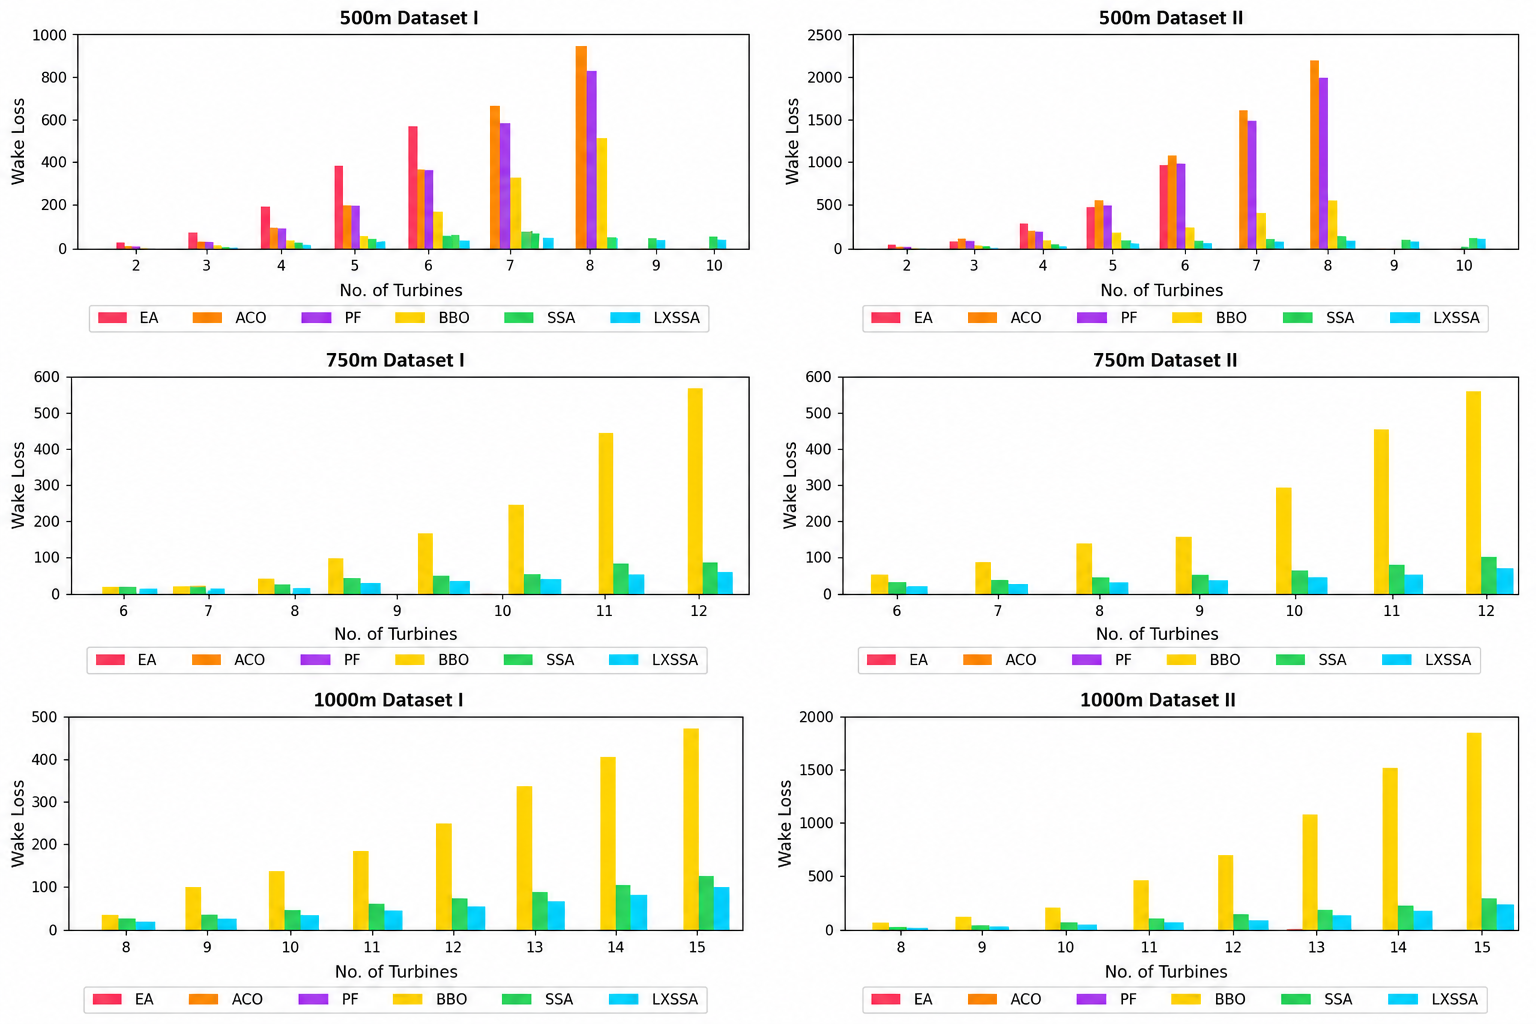
\includegraphics[width=\textwidth]{wake loss for 6 cases.png}
\caption{Comparison of wake loss values for different optimization algorithms across 500~m, 750~m, and 1000~m cases under Dataset I and Dataset II configurations.}
\label{fig:wakelosscomparison}
\end{figure*}

%%%%%%%%%%%%%%%%%%%%%%%%%%%%%%%%%%%%%%%%%%%%%%%%%%%%%%%%%%%%%

\subsection{Supplementary run-level comparison from the DS1/DS2 Paper1 workbooks}
\label{sec:additional-runlevel}
The separately supplied DS1 Paper1 and DS2 Paper1 workbooks contain 30 records per algorithm and case for SSA, LX-SSA, PSO and DE. The results below constitute a \emph{separate follow-up experiment}; they do not replace or extend the 30-run samples behind Tables~\ref{tab:500mI}--\ref{tab:1000mII}, whose reported means are different. For example, the Dataset~I, 500-m, four-turbine LX-SSA mean is 56080.34 in the new workbook and 56179.90 in Table~\ref{tab:500mI}. These distinct archives must not be pooled. The workbook labels are mapped to the manuscript's two synthetic wind datasets using their dataset fields; the reported power and wake-loss fields are retained in their original benchmark-objective units, not converted into annual energy production.

For a transparent, focused comparison, we selected three representative radius--turbine cases after reviewing geometric feasibility: 500~m/4, 750~m/8, and 1000~m/8 in each dataset. This post hoc selection makes all reported tests exploratory. All 30 recorded final layouts per algorithm in these six cases have the stated number of coordinates, remain within the specified circular boundary and satisfy the 308~m minimum center-to-center distance (verified directly from the stored coordinates with a $10^{-6}$~m numerical tolerance). This selection avoids treating the very large penalized loss values of infeasible runs in more crowded cases as physical wake losses. The full source workbooks also contain cases beyond the turbine-count ranges shown in the historical tables; those cases are not silently added to the historical experiment. The selected run records and coordinate strings accompany the revision as machine-readable data.

\begin{table*}[!t]
\centering\caption{Separate DS1/DS2 follow-up experiment: reported benchmark power objective, 30 runs per algorithm and case; mean $\pm$ sample SD. The evaluations column records objective calls per run; the time column is the recorded batch time divided by 30 (seconds per run), not an independently timed run, and the hardware of the recorded runs is undocumented.}
\label{tab:followup-results}
\footnotesize\setlength{\tabcolsep}{3pt}
\begin{tabular}{ccccccc}
\toprule
Dataset & Radius (m) & Turbines & Algorithm & Power objective (mean $\pm$ SD) & Evaluations & Time/run (s) \\
\midrule
1 & 500 & 4 & LX-SSA & $56080.34 \pm 19.54$ & 6,030 & 0.1456 \\
1 & 500 & 4 & SSA & $56082.40 \pm 21.77$ & 3,030 & 0.0354 \\
1 & 500 & 4 & PSO & $56073.17 \pm 13.26$ & 3,030 & 0.0094 \\
1 & 500 & 4 & DE & $56037.54 \pm 21.96$ & 3,030 & 0.0127 \\
\midrule
1 & 750 & 8 & LX-SSA & $111434.97 \pm 436.06$ & 6,030 & 0.1456 \\
1 & 750 & 8 & SSA & $111270.52 \pm 613.40$ & 3,030 & 0.0136 \\
1 & 750 & 8 & PSO & $110713.37 \pm 959.37$ & 3,030 & 0.0100 \\
1 & 750 & 8 & DE & $109402.64 \pm 871.97$ & 3,030 & 0.0120 \\
\midrule
1 & 1000 & 8 & LX-SSA & $111927.21 \pm 153.38$ & 6,030 & 0.1404 \\
1 & 1000 & 8 & SSA & $111886.13 \pm 224.57$ & 3,030 & 0.0129 \\
1 & 1000 & 8 & PSO & $111744.35 \pm 186.53$ & 3,030 & 0.0096 \\
1 & 1000 & 8 & DE & $111333.80 \pm 284.14$ & 3,030 & 0.0122 \\
\midrule
2 & 500 & 4 & LX-SSA & $29024.39 \pm 76.99$ & 6,030 & 0.1443 \\
2 & 500 & 4 & SSA & $28971.66 \pm 67.38$ & 3,030 & 0.0356 \\
2 & 500 & 4 & PSO & $29023.49 \pm 59.60$ & 3,030 & 0.0100 \\
2 & 500 & 4 & DE & $28897.19 \pm 82.42$ & 3,030 & 0.0118 \\
\midrule
2 & 750 & 8 & LX-SSA & $56708.27 \pm 361.39$ & 6,030 & 0.1458 \\
2 & 750 & 8 & SSA & $56620.38 \pm 325.74$ & 3,030 & 0.0134 \\
2 & 750 & 8 & PSO & $56325.33 \pm 515.72$ & 3,030 & 0.0096 \\
2 & 750 & 8 & DE & $55567.25 \pm 527.75$ & 3,030 & 0.0125 \\
\midrule
2 & 1000 & 8 & LX-SSA & $57661.26 \pm 207.06$ & 6,030 & 0.1453 \\
2 & 1000 & 8 & SSA & $57506.61 \pm 248.37$ & 3,030 & 0.0369 \\
2 & 1000 & 8 & PSO & $57398.25 \pm 218.65$ & 3,030 & 0.0096 \\
2 & 1000 & 8 & DE & $56985.58 \pm 157.92$ & 3,030 & 0.0124 \\

\bottomrule
\end{tabular}
\end{table*}

\begin{figure*}[!t]
\centering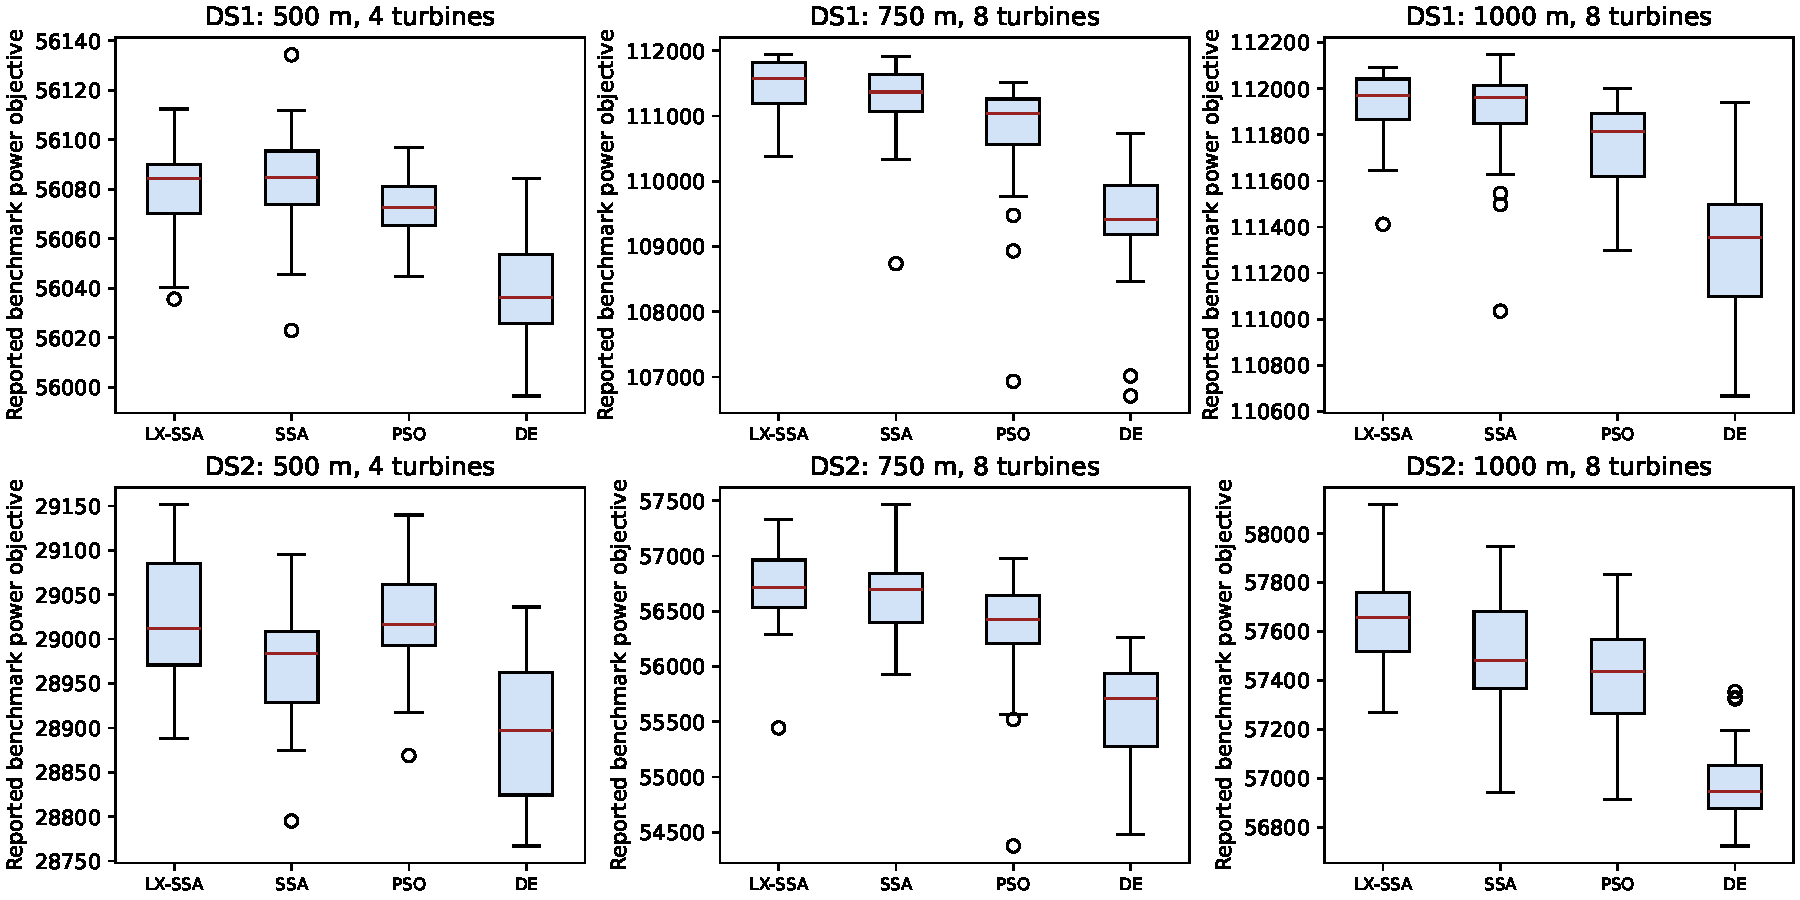
\includegraphics[width=\textwidth]{selected_power_boxplots.pdf}
\caption{Run-level distributions of the reported power objective in the six selected follow-up cases. Each box contains 30 runs. Comparisons are descriptive because LX-SSA has twice as many recorded objective evaluations as the other algorithms.}
\label{fig:selected-boxplots}
\end{figure*}

In the reported final-solution data, LX-SSA used 6,030 objective evaluations per run; SSA, PSO and DE each used 3,030. The common iteration cap (100) therefore did \emph{not} produce an equal objective-evaluation budget. Table~\ref{tab:followup-results} and Fig.~\ref{fig:selected-boxplots} describe performance at these \emph{different budgets}; neither should be read as evidence of better performance at equal computational cost. These counts are arithmetically consistent with a population of 30 salps/particles/individuals and 100 iterations ($30+100\times30=3030$) and, for LX-SSA, with two objective evaluations per population member per iteration ($30+100\times60=6030$); the follow-up population size therefore differs from the $N_p=5\times2N$ rule used for the historical tables. The repeated runtime field contains a single batch-level measurement divided by 30 for each algorithm/case, not 30 independent timings. These batch averages (last column of Table~\ref{tab:followup-results}) are 0.140--0.146~s per LX-SSA run versus 0.013--0.037~s for SSA and about 0.01~s for PSO and DE, i.e., LX-SSA was roughly 4--15 times slower per run in the recorded batches, more than its twofold evaluation count alone would explain. Because the hardware and software environment of these batches are undocumented and the values are not independent replicates, we report them descriptively and do not conduct runtime hypothesis tests.

The distributions were tested using an independent-sample Kruskal--Wallis test within each case, followed by two-sided Mann--Whitney tests comparing LX-SSA with each of SSA, PSO and DE; the three comparisons \emph{within each case} were adjusted by Holm's procedure. Positive mean differences and positive rank-biserial effects favor LX-SSA on the reported power objective. The seed labels alone do not establish matched initial conditions or paired random streams, so a paired signed-rank test is not justified. These tests describe differences in the \emph{recorded unequal-budget runs}; they do not remove the evaluation-budget confounding. We do not use the workbooks' all-algorithm Friedman/Wilcoxon summaries, which involve additional algorithms and assume a run-level pairing that the supplied metadata do not establish. Instead, following the multi-problem protocol of Dem\v{s}ar~\cite{Demsar2006}, a Friedman test is applied at the \emph{case level}: the six selected cases are the blocks and the four algorithms are ranked within each case by their mean objective, which requires no pairing of individual runs. Post hoc comparisons of LX-SSA with each baseline use the average-rank $z$ statistic with Holm correction~\cite{Holm1979}. Effect sizes are reported as rank-biserial correlations $r_{rb}=2A_{12}-1$, where $A_{12}$ is the Vargha--Delaney probability of superiority~\cite{Vargha2000}, and uncertainty in the mean difference is reported by bootstrap confidence intervals.

\begin{table*}[!t]
\centering\caption{Exploratory independent-sample tests for the selected follow-up cases. $H$ and $p_{\rm KW}$ are the four-algorithm Kruskal--Wallis statistic and $p$ value. The three adjusted $p$ values compare LX-SSA with each baseline using Mann--Whitney tests with Holm correction within the case. The 95\% CI of $\Delta$ is a percentile bootstrap interval (10{,}000 resamples) for the difference of means (LX-SSA minus baseline). Additional numerical precision for the $p$ values is provided in the accompanying analysis CSV; these are conventional asymptotic test $p$ values, not exact enumeration.}
\label{tab:exploratory-tests}
\footnotesize\setlength{\tabcolsep}{3pt}
\begin{tabular}{cccccccccc}
\toprule
DS & Radius (m) & $N$ & $H$ & $p_{\rm KW}$ & Baseline & $\Delta$ power & 95\% CI of $\Delta$ & $p_{\rm Holm}$ & Rank-biserial \\
\midrule
1 & 500 & 4 & 52.21 & $2.7\times10^{-11}$ & SSA & -2.06 & [-12.4, 8.1] & 0.6735 & -0.06 \\
1 & 500 & 4 & 52.21 & $2.7\times10^{-11}$ & PSO & +7.17 & [-1.3, 15.5] & 0.09029 & +0.30 \\
1 & 500 & 4 & 52.21 & $2.7\times10^{-11}$ & DE & +42.80 & [32.3, 53.2] & $4.29\times10^{-8}$ & +0.85 \\
\midrule
1 & 750 & 8 & 67.42 & $1.52\times10^{-14}$ & SSA & +164.45 & [-83.0, 439.7] & 0.2398 & +0.18 \\
1 & 750 & 8 & 67.42 & $1.52\times10^{-14}$ & PSO & +721.60 & [378.0, 1116.9] & $7.66\times10^{-5}$ & +0.62 \\
1 & 750 & 8 & 67.42 & $1.52\times10^{-14}$ & DE & +2032.33 & [1699.6, 2383.0] & $1.49\times10^{-10}$ & +0.99 \\
\midrule
1 & 1000 & 8 & 61.68 & $2.57\times10^{-13}$ & SSA & +41.08 & [-50.2, 141.1] & 0.5895 & +0.08 \\
1 & 1000 & 8 & 61.68 & $2.57\times10^{-13}$ & PSO & +182.87 & [97.0, 266.2] & $8.71\times10^{-5}$ & +0.62 \\
1 & 1000 & 8 & 61.68 & $2.57\times10^{-13}$ & DE & +593.41 & [480.2, 707.3] & $2.43\times10^{-9}$ & +0.92 \\
\midrule
2 & 500 & 4 & 38.23 & $2.53\times10^{-8}$ & SSA & +52.72 & [16.8, 89.0] & 0.03391 & +0.36 \\
2 & 500 & 4 & 38.23 & $2.53\times10^{-8}$ & PSO & +0.90 & [-32.6, 34.7] & 0.8303 & -0.03 \\
2 & 500 & 4 & 38.23 & $2.53\times10^{-8}$ & DE & +127.20 & [87.4, 167.2] & $6.46\times10^{-6}$ & +0.71 \\
\midrule
2 & 750 & 8 & 63.06 & $1.3\times10^{-13}$ & SSA & +87.89 & [-87.4, 251.3] & 0.3042 & +0.16 \\
2 & 750 & 8 & 63.06 & $1.3\times10^{-13}$ & PSO & +382.94 & [176.8, 610.9] & 0.001175 & +0.52 \\
2 & 750 & 8 & 63.06 & $1.3\times10^{-13}$ & DE & +1141.03 & [918.3, 1373.3] & $5.87\times10^{-10}$ & +0.96 \\
\midrule
2 & 1000 & 8 & 66.62 & $2.26\times10^{-14}$ & SSA & +154.65 & [43.7, 269.9] & 0.01988 & +0.35 \\
2 & 1000 & 8 & 66.62 & $2.26\times10^{-14}$ & PSO & +263.01 & [157.3, 371.5] & $8.17\times10^{-5}$ & +0.62 \\
2 & 1000 & 8 & 66.62 & $2.26\times10^{-14}$ & DE & +675.68 & [586.4, 768.4] & $1.65\times10^{-10}$ & +0.99 \\

\bottomrule
\end{tabular}
\end{table*}

\begin{table}[!t]
\centering
\caption{Case-level Friedman analysis of the four follow-up algorithms (blocks: the six selected cases; ranks computed from case means, 1 = highest objective). Post hoc $p$ values compare LX-SSA with each baseline and are Holm-adjusted.}
\label{tab:friedman}
\footnotesize
\begin{tabular}{lccc}
\toprule
Algorithm & Average rank & $z$ vs.\ LX-SSA & $p_{\rm Holm}$ \\
\midrule
LX-SSA & 1.17 & -- & -- \\
SSA & 2.00 & 1.118 & 0.264 \\
PSO & 2.83 & 2.236 & 0.0507 \\
DE & 4.00 & 3.801 & $4.32\times10^{-4}$ \\
\midrule
\multicolumn{4}{l}{Friedman $\chi^2_F=15.80$ (3 d.f.), $p=1.25\times10^{-3}$} \\
\multicolumn{4}{l}{Iman--Davenport $F_F=35.91$} \\
\bottomrule
\end{tabular}
\end{table}

Table~\ref{tab:friedman} shows that the four algorithms are not ranked equally across the selected cases ($\chi^2_F=15.80$, $p=0.0012$). LX-SSA has the best average rank (1.17; first in five cases and second in Dataset~I, 500~m/4), but after Holm correction only the difference from DE is significant ($p_{\rm Holm}=4.3\times10^{-4}$); the differences from PSO ($p_{\rm Holm}=0.051$) and SSA ($p_{\rm Holm}=0.26$) are not. With only six blocks the case-level test has low power, and the cases were selected post hoc, so these results are exploratory. They agree with the run-level analysis of the recorded data: across the 18 LX-SSA--baseline comparisons in Table~\ref{tab:exploratory-tests}, the Holm-adjusted test does not distinguish LX-SSA from its comparator at the 5\% level in six (SSA in Dataset~I at 500~m/4, 750~m/8 and 1000~m/8 and in Dataset~II at 750~m/8; PSO at 500~m/4 in both datasets), and the bootstrap intervals of $\Delta$ against SSA include zero in four of the six cases. The practically relevant effect sizes are therefore large against DE ($r_{rb}\geq0.71$), moderate against PSO in the 8-turbine cases ($r_{rb}\approx0.52$--$0.62$), and small against SSA ($|r_{rb}|\leq0.36$). All of these recorded comparisons, however, give LX-SSA twice the evaluation budget; Section~\ref{sec:equalbudget} shows that the advantage over SSA and PSO disappears at equal cost.

The selected results show a mixed mechanism-level comparison. For Dataset~I at 500~m/4, SSA exceeds LX-SSA by 2.06 objective units in sample mean and the Holm-adjusted comparison does not distinguish their run distributions ($p=0.6735$). At 750~m/8, the LX-SSA mean exceeds SSA by 164.45 and 87.89 units for Datasets~I and II, respectively, while neither SSA comparison survives the within-case Holm adjustment ($p=0.2398$ and $p=0.3042$). Dataset~II at 1000~m/8 shows a higher LX-SSA mean than SSA by 154.65 units ($p_{\mathrm{Holm}}=0.01988$); this difference remains confounded by LX-SSA's larger evaluation budget. The larger observed differences against DE and PSO cannot establish relative efficiency under equal computational effort.

These post hoc, unequal-budget tests are a limited diagnostic, not a basis for a universal superiority claim. In more crowded cases, the workbooks contain infeasible layouts with penalty-scale values in the \texttt{WakeLoss} column; reporting those raw means as physical wake deficits would be misleading. Section~\ref{sec:equalbudget} therefore repeats the comparison with the original code at equal budgets, seed-paired initial populations and full feasibility reporting.

\section{Controlled Re-runs with the Original Implementation}
\label{sec:equalbudget}
The follow-up data of Section~\ref{sec:additional-runlevel} compare algorithms at unequal budgets. To remove this confound, the original implementations of SSA, LX-SSA, PSO and DE, i.e., the code that produced the follow-up data, were re-run on the validated evaluator of Section~\ref{sec:validation} with the penalized objective~\eqref{eq:penalty}.

\subsection{Protocol and Calibration}
\label{sec:rerun-protocol}
\emph{Calibration.} At the recorded budgets (6,030 calls for LX-SSA, 3,030 for the others), the re-runs reproduce the recorded follow-up distributions. In 22 of the 24 algorithm--case comparisons, a Mann--Whitney test does not distinguish re-run from recorded objective values at the 5\% level (smallest $p=0.0015$, for SSA in Data Set~I at 500~m/4), and the largest relative difference between re-run and recorded means is 0.22\%. The counted objective calls are exactly 3,030 and 6,030, as recorded. This confirms that the reported LX-SSA results correspond to $\phi=0$ and $\chi=1$. One difference remains: in the 750-m eight-turbine cases, 22 (PSO) and 26 (DE) of the 30 re-runs end feasible, whereas all recorded runs in these cases were feasible.

\emph{Design.} Each algorithm uses a population of 30 and seeds 1--30. Every optimizer seeds the random-number generator and draws its initial population first, so runs with the same seed start from the \emph{same} initial population for all four algorithms (verified numerically). The runs are therefore paired by seed, which justifies the Wilcoxon signed-rank and run-level Friedman tests that the independent-sample analysis of Section~\ref{sec:additional-runlevel} could not use. Two budgets are matched in counted objective calls: 3,030 (LX-SSA 50 iterations; SSA, PSO and DE 100) and 6,030 (LX-SSA 100 iterations; the others 200). For ranking, a feasible run beats an infeasible one; infeasible runs are compared by their spacing shortfall.

\subsection{Equal-Budget Comparison}
\begin{table*}[!t]
\centering
\caption{Controlled equal-budget re-runs with the authors' optimizer code: benchmark objective (mean $\pm$ SD of the feasible runs among 30 seed-paired runs). Budget = objective-function calls per run (LX-SSA 50 or 100 iterations; SSA, PSO and DE 100 or 200 iterations; population 30). Bold: highest mean. A superscript gives the number of feasible runs when fewer than 30; infeasible runs are excluded from the mean.}
\label{tab:equalbudget}
\footnotesize\setlength{\tabcolsep}{4pt}
\begin{tabular}{cccccccc}
\toprule
Budget & DS & Radius (m) & $N$ & LX-SSA & SSA & PSO & DE \\
\midrule
3,030 & 1 & 500 & 4 & 56070.0 $\pm$ 20.3 & 56061.7 $\pm$ 25.0 & \textbf{56080.4 $\pm$ 19.4} & 56045.1 $\pm$ 16.5 \\
3,030 & 1 & 750 & 8 & 111322.4 $\pm$ 445.1 & \textbf{111383.2 $\pm$ 419.0} & 110839.7 $\pm$ 982.4$^{22}$ & 109724.0 $\pm$ 915.4$^{26}$ \\
3,030 & 1 & 1000 & 8 & 111791.5 $\pm$ 217.3 & \textbf{111860.0 $\pm$ 165.3} & 111719.0 $\pm$ 426.8$^{29}$ & 111402.9 $\pm$ 204.1 \\
3,030 & 2 & 500 & 4 & 28966.6 $\pm$ 91.8 & 28957.2 $\pm$ 92.7 & \textbf{29031.6 $\pm$ 49.6} & 28923.9 $\pm$ 86.9 \\
3,030 & 2 & 750 & 8 & 56567.9 $\pm$ 377.6 & \textbf{56744.1 $\pm$ 295.3} & 56370.7 $\pm$ 465.1$^{22}$ & 55520.8 $\pm$ 573.2$^{26}$ \\
3,030 & 2 & 1000 & 8 & \textbf{57564.8 $\pm$ 215.3} & 57545.6 $\pm$ 220.5 & 57376.6 $\pm$ 192.2$^{29}$ & 56984.8 $\pm$ 143.6 \\
\midrule
6,030 & 1 & 500 & 4 & 56078.3 $\pm$ 26.4 & 56085.5 $\pm$ 18.7 & \textbf{56094.4 $\pm$ 12.3} & 56082.2 $\pm$ 26.4 \\
6,030 & 1 & 750 & 8 & 111455.0 $\pm$ 284.4 & \textbf{111599.1 $\pm$ 314.1} & 111313.6 $\pm$ 718.6$^{29}$ & 110464.8 $\pm$ 657.0 \\
6,030 & 1 & 1000 & 8 & 111896.7 $\pm$ 145.8 & \textbf{111942.7 $\pm$ 87.4} & 111932.8 $\pm$ 152.3 & 111566.5 $\pm$ 182.4 \\
6,030 & 2 & 500 & 4 & 29016.4 $\pm$ 68.3 & 28994.0 $\pm$ 65.8 & \textbf{29099.1 $\pm$ 65.2} & 29049.7 $\pm$ 85.8 \\
6,030 & 2 & 750 & 8 & 56709.7 $\pm$ 231.9 & \textbf{56805.1 $\pm$ 308.6} & 56804.1 $\pm$ 259.8$^{29}$ & 56104.7 $\pm$ 378.0 \\
6,030 & 2 & 1000 & 8 & 57535.3 $\pm$ 200.3 & \textbf{57707.4 $\pm$ 182.0} & 57645.8 $\pm$ 228.6 & 57146.1 $\pm$ 177.0 \\
\bottomrule
\end{tabular}
\end{table*}


\begin{table*}[!t]
\centering
\caption{Paired statistics for the equal-budget re-runs (runs paired by seed, i.e., by identical initial population). $\chi^2_F$, $p_F$: run-level Friedman test over the four algorithms (30 blocks); $\bar r$: average Friedman rank of LX-SSA (1 = best). Infeasible runs rank below feasible ones (and among themselves by spacing shortfall). For each baseline: difference of feasible-run means (LX-SSA minus baseline), LX-SSA wins/losses over the 30 pairs, Holm-adjusted two-sided Wilcoxon signed-rank $p$, and matched-pairs rank-biserial correlation (positive favors LX-SSA).}
\label{tab:equalbudget-tests}
\scriptsize\setlength{\tabcolsep}{3pt}
\begin{tabular}{cccccccccccc}
\toprule
Budget & DS & Radius & $N$ & $\chi^2_F$ & $p_F$ & $\bar r$ & Baseline & $\Delta$ & W/L & $p_{\rm Holm}$ & $r_{rb}$ \\
\midrule
3,030 & 1 & 500 & 4 & 29.32 & $1.92\times10^{-6}$ & 2.30 & SSA & +8.3 & 16/14 & 0.371 & +0.19 \\
 & & & & & &  & PSO & -10.4 & 10/20 & 0.168 & -0.36 \\
 & & & & & &  & DE & +24.8 & 25/5 & $3.18\times10^{-5}$ & +0.84 \\
\midrule
3,030 & 1 & 750 & 8 & 36.68 & $5.38\times10^{-8}$ & 1.87 & SSA & -60.8 & 15/15 & 0.543 & -0.13 \\
 & & & & & &  & PSO & +482.7 & 19/11 & 0.002 & +0.66 \\
 & & & & & &  & DE & +1598.4 & 30/0 & $5.59\times10^{-9}$ & +1.00 \\
\midrule
3,030 & 1 & 1000 & 8 & 42.12 & $3.78\times10^{-9}$ & 2.13 & SSA & -68.5 & 13/17 & 0.382 & -0.28 \\
 & & & & & &  & PSO & +72.5 & 16/14 & 0.382 & +0.22 \\
 & & & & & &  & DE & +388.6 & 27/3 & $1.06\times10^{-7}$ & +0.97 \\
\midrule
3,030 & 2 & 500 & 4 & 26.12 & $9.00\times10^{-6}$ & 2.53 & SSA & +9.4 & 17/13 & 0.543 & +0.13 \\
 & & & & & &  & PSO & -65.0 & 8/22 & 0.014 & -0.58 \\
 & & & & & &  & DE & +42.7 & 19/11 & 0.168 & +0.36 \\
\midrule
3,030 & 2 & 750 & 8 & 46.52 & $4.40\times10^{-10}$ & 2.03 & SSA & -176.2 & 10/20 & 0.084 & -0.36 \\
 & & & & & &  & PSO & +197.1 & 21/9 & 0.001 & +0.69 \\
 & & & & & &  & DE & +1047.1 & 28/2 & $2.79\times10^{-8}$ & +0.99 \\
\midrule
3,030 & 2 & 1000 & 8 & 52.44 & $2.41\times10^{-11}$ & 1.70 & SSA & +19.1 & 15/15 & 0.839 & +0.05 \\
 & & & & & &  & PSO & +188.1 & 24/6 & 0.001 & +0.69 \\
 & & & & & &  & DE & +580.0 & 30/0 & $5.59\times10^{-9}$ & +1.00 \\
\midrule
6,030 & 1 & 500 & 4 & 8.80 & 0.032 & 2.77 & SSA & -7.3 & 14/16 & 0.929 & -0.16 \\
 & & & & & &  & PSO & -16.1 & 9/21 & 0.011 & -0.59 \\
 & & & & & &  & DE & -3.9 & 14/16 & 0.929 & -0.07 \\
\midrule
6,030 & 1 & 750 & 8 & 39.92 & $1.11\times10^{-8}$ & 2.27 & SSA & -144.1 & 9/21 & 0.050 & -0.47 \\
 & & & & & &  & PSO & +141.4 & 15/15 & 0.428 & +0.17 \\
 & & & & & &  & DE & +990.2 & 28/2 & $2.79\times10^{-8}$ & +0.99 \\
\midrule
6,030 & 1 & 1000 & 8 & 49.68 & $9.35\times10^{-11}$ & 2.13 & SSA & -46.0 & 14/16 & 0.457 & -0.26 \\
 & & & & & &  & PSO & -36.2 & 12/18 & 0.457 & -0.20 \\
 & & & & & &  & DE & +330.2 & 30/0 & $5.59\times10^{-9}$ & +1.00 \\
\midrule
6,030 & 2 & 500 & 4 & 25.20 & $1.40\times10^{-5}$ & 2.80 & SSA & +22.4 & 17/13 & 0.368 & +0.28 \\
 & & & & & &  & PSO & -82.6 & 6/24 & $3.18\times10^{-5}$ & -0.84 \\
 & & & & & &  & DE & -33.3 & 13/17 & 0.368 & -0.28 \\
\midrule
6,030 & 2 & 750 & 8 & 34.36 & $1.66\times10^{-7}$ & 2.33 & SSA & -95.4 & 13/17 & 0.396 & -0.27 \\
 & & & & & &  & PSO & -94.4 & 12/18 & 0.396 & -0.23 \\
 & & & & & &  & DE & +605.1 & 25/5 & $2.50\times10^{-6}$ & +0.91 \\
\midrule
6,030 & 2 & 1000 & 8 & 55.64 & $5.01\times10^{-12}$ & 2.47 & SSA & -172.1 & 8/22 & 0.011 & -0.57 \\
 & & & & & &  & PSO & -110.4 & 8/22 & 0.014 & -0.51 \\
 & & & & & &  & DE & +389.2 & 30/0 & $5.59\times10^{-9}$ & +1.00 \\
\bottomrule
\end{tabular}
\end{table*}


Tables~\ref{tab:equalbudget} and~\ref{tab:equalbudget-tests} show that the advantage of LX-SSA seen at unequal budgets does not persist at equal cost:
\begin{itemize}
\item \emph{LX-SSA vs.\ SSA (mechanism-level ablation).} At 3,030 calls the Holm-adjusted Wilcoxon test finds no difference in any of the six cases. At 6,030 calls SSA has the higher mean in five of six cases and is significantly better in two (Data Set~I, 750~m/8, $p_{\rm Holm}=0.050$; Data Set~II, 1000~m/8, $p_{\rm Holm}=0.011$). Under an equal number of objective calls, the Laplace follower candidate therefore does not improve on the SSA follower update for this problem. A plausible reason is that LX-SSA spends two calls per follower per iteration, so at a fixed budget it performs only half as many iterations.
\item \emph{LX-SSA vs.\ PSO.} At 3,030 calls LX-SSA is significantly better in three of the four eight-turbine cases, and PSO is better in Data Set~II at 500~m/4. At 6,030 calls PSO is significantly better in three cases (both 500~m/4 cases and Data Set~II at 1000~m/8), with no significant difference in the other three.
\item \emph{LX-SSA vs.\ DE.} LX-SSA is significantly better in five of six cases at 3,030 calls and in all four eight-turbine cases at 6,030 calls, with large effects ($r_{rb}\ge0.84$); the four-turbine cases show no significant difference at 6,030 calls.
\end{itemize}
Averaged over the six cases, the Friedman rank of LX-SSA is 2.09 at 3,030 calls (SSA 2.05, PSO 2.26, DE 3.59) and 2.46 at 6,030 calls (PSO 1.96, SSA 2.18, DE 3.39). LX-SSA is thus competitive with SSA and PSO and clearly better than DE, but equal-budget evidence does not support a claim that it outperforms SSA or PSO on this benchmark.

\subsection{Crowded Cases and Feasibility}
\begin{table*}[!t]
\centering
\caption{Equal-budget re-runs (6,030 calls) for the largest turbine count tabulated per radius: number of feasible final layouts out of 30 and mean benchmark objective of the feasible layouts.}
\label{tab:crowded}
\footnotesize\setlength{\tabcolsep}{4pt}
\begin{tabular}{ccccccccccc}
\toprule
& & & \multicolumn{2}{c}{LX-SSA} & \multicolumn{2}{c}{SSA} & \multicolumn{2}{c}{PSO} & \multicolumn{2}{c}{DE} \\
\cmidrule(lr){4-5}\cmidrule(lr){6-7}\cmidrule(lr){8-9}\cmidrule(lr){10-11}
DS & Radius (m) & $N$ & Feas. & Objective & Feas. & Objective & Feas. & Objective & Feas. & Objective \\
\midrule
1 & 500 & 10 & 22/30 & 131797.3 & 25/30 & 133122.8 & 0/30 & -- & 2/30 & 135428.3 \\
1 & 750 & 12 & 30/30 & 162767.5 & 30/30 & 163670.7 & 2/30 & 162719.7 & 0/30 & -- \\
1 & 1000 & 15 & 30/30 & 204425.3 & 30/30 & 204948.8 & 0/30 & -- & 1/30 & 204165.1 \\
2 & 500 & 10 & 22/30 & 66101.5 & 25/30 & 66447.2 & 0/30 & -- & 2/30 & 67317.9 \\
2 & 750 & 12 & 30/30 & 81808.7 & 30/30 & 82320.7 & 2/30 & 81921.7 & 0/30 & -- \\
2 & 1000 & 15 & 30/30 & 102880.2 & 30/30 & 103132.5 & 0/30 & -- & 1/30 & 102934.8 \\
\bottomrule
\end{tabular}
\end{table*}


For the largest turbine count of each historical table, Table~\ref{tab:crowded} reports how often each algorithm returns a feasible layout at 6,030 calls. The two salp-swarm algorithms are far more reliable than PSO and DE: LX-SSA and SSA return feasible layouts in 22--30 and 25--30 of 30 runs, respectively, whereas PSO and DE succeed in at most two runs per case. This feasibility advantage of the SSA family is the most robust practical difference observed. Between the two, SSA attains the higher mean objective among feasible runs in all six crowded cases.

\subsection{Measured Wind Climate: Horns Rev 1}
\label{sec:hornsrev}
\begin{table*}[!t]
\centering
\caption{Measured wind climate (Horns Rev~1 wind rose, 12 sectors): expected farm power in kW (mean $\pm$ SD of the feasible runs among 30 seed-paired runs, 6,030 calls each; a superscript gives the number of feasible runs when fewer than 30; AEP in MWh $=8.76\times$ kW). ``Ideal'' is the wake-free farm power. Bold: highest mean. $p_F$: run-level Friedman test; last three columns: Holm-adjusted Wilcoxon signed-rank $p$ of LX-SSA vs.\ SSA, PSO and DE.}
\label{tab:hornsrev}
\footnotesize\setlength{\tabcolsep}{3pt}
\begin{tabular}{cccccccccccc}
\toprule
& & & & & & & & \multicolumn{3}{c}{LX-SSA vs.\ ($p_{\rm Holm}$)} \\
\cmidrule(lr){9-11}
Radius (m) & $N$ & Ideal & LX-SSA & SSA & PSO & DE & $p_F$ & SSA & PSO & DE \\
\midrule
500 & 4 & 3157.9 & 3155.5 $\pm$ 5.0 & 3157.5 $\pm$ 1.8 & \textbf{3157.9 $\pm$ 0.0} & 3157.9 $\pm$ 0.0 & 0.003 & 0.109 & 0.094 & 0.094 \\
750 & 8 & 6315.7 & 6240.1 $\pm$ 32.8 & \textbf{6248.0 $\pm$ 26.5} & 6211.7 $\pm$ 53.6$^{29}$ & 6116.4 $\pm$ 69.9 & $3.64\times10^{-9}$ & 0.328 & 0.020 & $1.40\times10^{-7}$ \\
1000 & 8 & 6315.7 & 6273.2 $\pm$ 19.8 & \textbf{6282.3 $\pm$ 15.4} & 6265.2 $\pm$ 18.9 & 6217.8 $\pm$ 23.1 & $3.18\times10^{-11}$ & 0.146 & 0.146 & $2.79\times10^{-8}$ \\
1000 & 15 & 11842.0 & 11279.6 $\pm$ 102.8 & \textbf{11367.5 $\pm$ 92.4} & --$^{0}$ & 11310.2$^{1}$ & $1.12\times10^{-15}$ & 0.002 & $5.59\times10^{-9}$ & $7.45\times10^{-9}$ \\
\bottomrule
\end{tabular}
\end{table*}

To address the use of synthetic wind data, the four algorithms were applied to the measured wind climate of the Horns Rev~1 offshore wind farm. The 12 directional sectors, with Weibull scale, shape and frequency per sector, are taken from the open-source PyWake distribution~\cite{PyWake}. Only the wind climate is site-measured: the benchmark turbine, the Jensen wake model and the circular farm are unchanged, so this is a test of the optimizers under a realistic, strongly directional wind rose rather than a reproduction of the Horns Rev~1 farm. The free-stream expected power is 789.5~kW per turbine (capacity factor 0.53 under the benchmark power curve).

Table~\ref{tab:hornsrev} shows the same pattern as the synthetic data. SSA has the highest mean in the three larger cases. LX-SSA does not differ significantly from SSA except for 1000~m/15, where SSA is better ($p_{\rm Holm}=0.002$; mean wake losses 4.75\% vs.\ 4.01\% of the ideal, i.e., AEP of 98.8 vs.\ 99.6~GWh). LX-SSA is significantly better than DE in the three larger cases and better than PSO at 750~m/8 and 1000~m/15; at 1000~m/15 PSO finds no feasible layout and DE only one. In the four-turbine case PSO and DE reach the wake-free optimum in every run, while LX-SSA falls short by 2.3~kW on average (not significant after correction).

\subsection{Measured Run Time}
Each run was timed individually. At equal numbers of objective calls the four algorithms take essentially the same time: 0.39--0.46~ms per call on average (LX-SSA 0.39, SSA 0.40, PSO 0.41, DE 0.46~ms), i.e., 1.8--3.6~s per 6,030-call run depending on $N$. The run time is dominated by the objective evaluation, and the Laplace step adds no measurable overhead. The large per-run differences in the recorded batch times of Table~\ref{tab:followup-results} (up to 15 times longer for LX-SSA) are therefore not reproduced and are attributable to the undocumented recording conditions rather than to the algorithms. Environment: Linux container, Intel Xeon processor at 2.80~GHz, 4 virtual cores with four runs executed in parallel, Python~3.11.15, NumPy~2.4.6, SciPy~1.17.1.

\subsection{Effect of Boundary Handling}
The implementation clips coordinates to the bounding square and penalizes points outside the circle (Section~\ref{sec:constraints}). An otherwise identical SSA that instead projects every turbine radially onto the circle and ranks candidates by the feasibility-first rules attains higher mean objectives than the SSA re-runs in all six representative cases at 3,030 calls (by 40 to 507 objective units; for example 111774.0 vs.\ 111383.2 for Data Set~I at 750~m/8). The boundary-handling rule therefore affects results by more than the differences between the algorithms, and it must be held fixed, as here, in any comparison.

\section{Robustness of the Benchmark Assumptions}
\label{sec:robustness}
The reviewers questioned three modeling choices inherited from the legacy benchmark: the piecewise-linear power curve, Jensen's wake model, and the $4D$ minimum spacing. This section tests how far the conclusions depend on them. Except for the spacing re-optimization in Section~\ref{sec:spacing}, every analysis below \emph{re-evaluates} the 720 stored final layouts of the follow-up experiment (Section~\ref{sec:additional-runlevel}); no layout is re-optimized, so these checks show how sensitive the reported numbers and the algorithm ordering are to the model, not how each algorithm would perform if it were optimized under the alternative model. The scripts and per-run outputs accompany the revision.

\subsection{Independent Evaluator and Its Validation}
\label{sec:validation}
The benchmark objective of Section~\ref{sec:powermodel}, with the wake geometry of Lemmas~1--2, root-sum-square superposition \eqref{eq5}, the Weibull scale transformation \eqref{eq:weibull-scale}, 24 direction bins and 0.5~m/s speed bins, was re-implemented independently of the code that produced the archived results. Applied to the stored coordinates of all 720 follow-up layouts, it reproduces the recorded objective values with a maximum absolute deviation of $8.7\times10^{-11}$ and the recorded wake losses with a maximum deviation of $2.4\times10^{-4}$ objective units. The evaluator is therefore numerically identical to the implementation behind the follow-up data, which also confirms the objective definition and the conversion to expected power and AEP stated in Section~\ref{sec:powermodel}. For Wind Data Set~II, the ideal objective implied by the follow-up data (14630.76 for two turbines) differs by 0.004\% from the historical tabulated value (14631.37), a minor difference that does not affect any conclusion.

\subsection{Nonlinear Power Curve}
\label{sec:powercurve}
\begin{table*}[!t]
\centering
\caption{Re-evaluation of the 720 stored follow-up layouts with a nonlinear (cubic) power curve. $\bar P$ is the mean expected farm power of the LX-SSA layouts in kW (objective/15). $\Delta_{\rm c}$ and $\Delta_{\rm co}$ are the relative changes of the mean expected power (range over the four algorithms) for the cubic curve without and with a 25~m/s cut-out. The last two columns list the algorithms in decreasing order of mean expected power.}
\label{tab:powercurve}
\footnotesize\setlength{\tabcolsep}{4pt}
\begin{tabular}{cccccccc}
\toprule
DS & Radius (m) & $N$ & $\bar P$ linear (kW) & $\bar P$ cubic (kW) & $\Delta_{\rm c}$ (\%) & $\Delta_{\rm co}$ (\%) & Order: linear $\rightarrow$ cubic \\
\midrule
1 & 500 & 4 & 3738.7 & 3087.0 & [-17.5, -17.4] & [-21.4, -21.4] & SSA, LX, PSO, DE $\rightarrow$ SSA, LX, PSO, DE \\
1 & 750 & 8 & 7429.0 & 6116.9 & [-18.3, -17.7] & [-21.8, -21.5] & LX, SSA, PSO, DE $\rightarrow$ LX, SSA, PSO, DE \\
1 & 1000 & 8 & 7461.8 & 6155.5 & [-17.7, -17.5] & [-21.5, -21.4] & LX, SSA, PSO, DE $\rightarrow$ LX, SSA, PSO, DE \\
2 & 500 & 4 & 1935.0 & 1230.2 & [-36.5, -36.4] & [-36.6, -36.6] & LX, PSO, SSA, DE $\rightarrow$ PSO, LX, SSA, DE \\
2 & 750 & 8 & 3780.6 & 2379.6 & [-37.6, -37.1] & [-37.7, -37.2] & LX, SSA, PSO, DE $\rightarrow$ LX, SSA, PSO, DE \\
2 & 1000 & 8 & 3844.1 & 2436.5 & [-36.9, -36.6] & [-37.1, -36.8] & LX, SSA, PSO, DE $\rightarrow$ LX, SSA, PSO, DE \\
\bottomrule
\end{tabular}
\end{table*}


To test the linear power segment in \eqref{eq7}, the stored layouts were re-evaluated with the cubic power-curve model~\cite{Carrillo2013}
\[
f_{\rm c}(s)=P_{\text{rated}}\,\frac{s^3-s_{\text{cut-in}}^3}{s_{\text{rated}}^3-s_{\text{cut-in}}^3},\qquad s_{\text{cut-in}}\le s\le s_{\text{rated}},
\]
with $f_{\rm c}=0$ below cut-in and $f_{\rm c}=P_{\text{rated}}$ above rated speed. The curve uses the same cut-in speed, rated speed and rated power as the benchmark, so it isolates the effect of the shape of the power curve. A second variant adds a 25~m/s cut-out. Expected values were computed by quadrature on a 0.01~m/s grid using the same wake-scaled Weibull distributions.

Table~\ref{tab:powercurve} shows that the linear benchmark curve substantially overstates expected power relative to the cubic curve: the free-stream expected power per turbine falls from 936.4 to 773.8~kW for Data Set~I ($-17.4\%$) and from 487.7 to 310.4~kW for Data Set~II ($-36.4\%$), and the farm-level reductions for the stored layouts are $-17.4\%$ to $-18.3\%$ and $-36.4\%$ to $-37.6\%$, respectively. Adding the cut-out mainly affects the high-wind Data Set~I ($-21.4\%$ to $-21.8\%$). The absolute energy values reported in this paper are therefore specific to the benchmark curve and should not be read as turbine-specific AEP estimates. The \emph{relative} comparison is much less sensitive: within each case the Spearman correlation between the linear and cubic objective values of the 120 stored layouts is at least 0.957, and the ordering of the four algorithms by mean expected power is unchanged in five of the six cases. The exception is Data Set~II at 500~m/4, where LX-SSA and PSO differ by only 0.9 objective units under the linear curve (a difference not distinguished by the tests of Table~\ref{tab:exploratory-tests}) and PSO ranks first under the cubic curve.

\subsection{Gaussian Wake Model}
\label{sec:gaussian}
\begin{table*}[!t]
\centering
\caption{Mean wake loss (benchmark-objective units) of the stored follow-up layouts under the Jensen model used for optimization and under the Gaussian model of Bastankhah and Port\'e-Agel ($k^*=0.04$), 30 layouts per algorithm and case. The layouts were optimized with the Jensen model and are only re-evaluated here.}
\label{tab:gaussian}
\footnotesize\setlength{\tabcolsep}{4pt}
\begin{tabular}{ccccccccccc}
\toprule
& & & \multicolumn{4}{c}{Jensen wake loss} & \multicolumn{4}{c}{Gaussian wake loss ($k^*=0.04$)} \\
\cmidrule(lr){4-7}\cmidrule(lr){8-11}
DS & Radius (m) & $N$ & LX-SSA & SSA & PSO & DE & LX-SSA & SSA & PSO & DE \\
\midrule
1 & 500 & 4 & 102.6 & \textbf{100.6} & 109.8 & 145.4 & 183.2 & \textbf{170.6} & 199.2 & 213.7 \\
1 & 750 & 8 & \textbf{930.9} & 1095.4 & 1652.5 & 2963.3 & \textbf{1369.4} & 1497.8 & 1719.9 & 3032.8 \\
1 & 1000 & 8 & \textbf{438.7} & 479.8 & 621.6 & 1032.1 & \textbf{674.6} & 752.0 & 786.9 & 1081.9 \\
2 & 500 & 4 & \textbf{237.1} & 289.8 & 238.0 & 364.3 & 332.3 & 351.7 & \textbf{316.9} & 430.7 \\
2 & 750 & 8 & \textbf{1814.8} & 1902.6 & 2197.7 & 2955.8 & \textbf{2111.0} & 2153.0 & 2254.7 & 2781.6 \\
2 & 1000 & 8 & \textbf{861.8} & 1016.4 & 1124.8 & 1537.4 & \textbf{1019.6} & 1226.5 & 1175.1 & 1531.5 \\
\bottomrule
\multicolumn{11}{l}{\footnotesize Bold: lowest mean wake loss in the case under the respective model.}
\end{tabular}
\end{table*}


The stored layouts were also re-evaluated with the Gaussian wake model of Bastankhah and Port\'e-Agel~\cite{Bastankhah2014}. For a downstream distance $x>0$ and radial offset $r_\perp$ from the wake centerline,
\begin{align*}
\delta_{ij}&=\left(1-\sqrt{1-\frac{C_T}{8(\sigma/D)^2}}\right)\exp\!\left(-\frac{r_\perp^2}{2\sigma^2}\right),\\
\frac{\sigma}{D}&=k^*\frac{x}{D}+0.2\sqrt{\beta},
\end{align*}
with $\beta=\tfrac12(1+\sqrt{1-C_T})/\sqrt{1-C_T}$. The deficit is evaluated at the rotor center and combined by the same root-sum-square superposition and Weibull scaling as the Jensen benchmark. The wake growth rate is $k^*=0.04$, with $k^*=0.022$ as a sensitivity value.

Table~\ref{tab:gaussian} shows that the Gaussian model assigns larger mean wake losses to the same layouts in 22 of the 24 algorithm--case combinations (the exceptions are DE in the 750-m and 1000-m cases of Data Set~II). This is expected, because layouts optimized with the Jensen model can exploit its sharp-edged wake cone and the 24 discrete direction bins by placing turbines just outside the modeled wakes, whereas the Gaussian deficit decays smoothly in the lateral direction. The within-case Spearman correlation between Jensen and Gaussian wake losses ranges from 0.38 (Data Set~I, 500~m/4) to 0.93, so the ranking of individual layouts can change noticeably. At the algorithm level, the algorithm with the lowest mean wake loss is the same under both models in five of six cases for $k^*=0.04$ and in all six cases for $k^*=0.022$; the only change is Data Set~II at 500~m/4, where PSO has the lowest Gaussian wake loss for $k^*=0.04$. The full four-algorithm ordering is preserved in four cases for $k^*=0.04$ and in five for $k^*=0.022$. Wake-loss differences between algorithms should therefore be read as properties of the Jensen benchmark; whether they persist when layouts are \emph{optimized} with a higher-fidelity wake model remains to be tested.

\subsection{Minimum-Spacing Sensitivity}
\label{sec:spacing}
\begin{table}[!t]
\centering
\caption{Largest turbine count for which a layout satisfying the circular boundary and the minimum spacing was constructed (multi-start packing search; a constructive lower bound on geometric capacity), compared with the largest $N$ in the historical tables.}
\label{tab:capacity}
\footnotesize
\begin{tabular}{ccccc}
\toprule
Radius (m) & $4D$ & $5D$ & $6D$ & Largest $N$ in \\
 & (308 m) & (385 m) & (462 m) & Tables~\ref{tab:500mI}--\ref{tab:1000mII} \\
\midrule
500 & 13 & 8 & 7 & 10 \\
750 & 26 & 19 & 13 & 12 \\
1000 & 42 & 29 & 21 & 15 \\
\bottomrule
\end{tabular}
\end{table}


\begin{table*}[!t]
\centering
\caption{Minimum-spacing sensitivity with the authors' LX-SSA and SSA code (6,030 calls, 30 seed-paired runs per cell): mean benchmark objective, Wilcoxon signed-rank $p$ for LX-SSA vs.\ SSA, and the mean LX-SSA wake loss as a percentage of the ideal objective at $4D$ and $6D$. A superscript gives the number of feasible runs when fewer than 30.}
\label{tab:spacing-authors}
\footnotesize\setlength{\tabcolsep}{3pt}
\begin{tabular}{ccccccccccccc}
\toprule
& & & \multicolumn{3}{c}{$4D$ (308 m)} & \multicolumn{3}{c}{$5D$ (385 m)} & \multicolumn{3}{c}{$6D$ (462 m)} & \\
\cmidrule(lr){4-6}\cmidrule(lr){7-9}\cmidrule(lr){10-12}
DS & Radius & $N$ & LX-SSA & SSA & $p$ & LX-SSA & SSA & $p$ & LX-SSA & SSA & $p$ & LX-SSA loss (\%) \\
\midrule
1 & 500 & 4 & 56078.3 & 56085.5 & 0.465 & 56082.4 & 56082.3 & 0.855 & 56071.5 & 56041.2 & 0.289 & 0.19 $\rightarrow$ 0.20 \\
1 & 750 & 8 & 111455.0 & 111599.1 & 0.025 & 111141.0 & 111435.3 & 0.064 & 110828.0 & 110896.1 & 0.808 & 0.81 $\rightarrow$ 1.37 \\
1 & 1000 & 8 & 111896.7 & 111942.7 & 0.229 & 111952.4 & 111894.4 & 0.730 & 111831.8 & 111878.7 & 0.318 & 0.42 $\rightarrow$ 0.48 \\
2 & 500 & 4 & 29016.4 & 28994.0 & 0.184 & 28964.7 & 28999.6 & 0.135 & 28996.7 & 28999.0 & 0.935 & 0.84 $\rightarrow$ 0.90 \\
2 & 750 & 8 & 56709.7 & 56805.1 & 0.198 & 56716.1 & 56773.2 & 0.570 & 56583.8 & 56790.0 & 0.007 & 3.10 $\rightarrow$ 3.31 \\
2 & 1000 & 8 & 57535.3 & 57707.4 & 0.005 & 57523.8 & 57566.5 & 0.404 & 57452.2 & 57546.5 & 0.088 & 1.69 $\rightarrow$ 1.83 \\
\bottomrule
\end{tabular}
\end{table*}

The spacing assumption was examined in three complementary ways.

\emph{Geometric capacity.} Table~\ref{tab:capacity} reports, for each radius and spacing, the largest turbine count for which a multi-start packing search constructed a layout satisfying both the circular boundary and the minimum distance. These are constructive lower bounds on the true geometric capacity; the 500-m values (13, 8 and 7) coincide with the known optimal circle-packing results. Under the benchmark $4D$ rule, all turbine counts in the historical tables (at most 10, 12 and 15 for the three radii) are far below the constructible capacity (13, 26 and 42), so those tables do not probe densely packed farms. The capacity falls steeply with spacing: for the 500-m farm it drops to 8 turbines at $5D$ and 7 at $6D$, so the tabulated 500-m cases with $N=9$--$10$ would be infeasible at $5D$ and those with $N=8$--$10$ at $6D$, whereas all tabulated 750-m and 1000-m cases remain geometrically feasible up to $6D$ (capacities 13 and 21).

\emph{Stored layouts.} The layouts optimized under $4D$ are frequently active at the spacing constraint. Of the 240 stored four-turbine layouts, 77.5\% also satisfy $5D$ and 40.4\% satisfy $6D$; of the 480 stored eight-turbine layouts, only 27.3\% satisfy $5D$ and 5.6\% satisfy $6D$ (none of the 750-m, eight-turbine layouts satisfies $6D$). The reported optimal layouts are therefore specific to the $4D$ rule and cannot be transferred to a site with larger spacing requirements without re-optimization.

\emph{Re-optimization.} The six representative cases were re-optimized with the original LX-SSA and SSA code at $5D$ and $6D$ (6,030 calls, 30 seed-paired runs; the $4D$ values are those of Section~\ref{sec:equalbudget}). All 720 re-optimized layouts are feasible. Table~\ref{tab:spacing-authors} shows that larger spacing has little effect in the four-turbine 500-m and eight-turbine 1000-m cases, but in the denser 750-m eight-turbine cases it lowers the mean LX-SSA objective from $4D$ to $6D$ by 627 units (0.56\%) for Data Set~I and 126 units (0.22\%) for Data Set~II, with the mean wake loss rising from 0.81\% to 1.37\% and from 3.10\% to 3.31\% of the ideal objective. The LX-SSA--SSA comparison is not reversed by the spacing rule: SSA has the higher mean in most cells, and the only significant differences (unadjusted Wilcoxon $p<0.05$) favor SSA, at $4D$ for Data Set~I at 750~m/8 and Data Set~II at 1000~m/8 and at $6D$ for Data Set~II at 750~m/8. Tighter spacing thus matters mainly for densely populated farms, which is exactly where the historical tables report their largest turbine counts.

\section{\textbf{Computational Complexity and Evidence Strength}}

\subsection{Asymptotic Computational Cost}
Let $N_t$ be the number of turbines, $N_p$ the population size, $d=2N_t$ the decision dimension, $T$ the number of iterations, $N_\theta$ the number of wind-direction bins, and $N_s$ the number of wind-speed bins. A direct wake evaluation contains pairwise turbine interactions and directional/speed discretization, giving the dominant objective cost
\[
C_{\mathrm{obj}}=\mathcal{O}\!\left(N_t^2N_\theta N_s\right).
\]
Evaluating all population members over $T$ iterations therefore gives
\[
\mathcal{O}\!\left(TN_pN_t^2N_\theta N_s\right).
\]
Boundary projection is $\mathcal{O}(N_t)$ per candidate and pairwise spacing evaluation is $\mathcal{O}(N_t^2)$; both are dominated by the wake/objective evaluation. The additional Laplace draw and candidate update in LX-SSA are linear in the decision dimension, so they do not change the leading asymptotic order relative to SSA. This is an asymptotic statement only; actual wall-clock overhead must be measured empirically.

\subsection{Run-to-Run Evidence and Statistical Limitations}
The historical six-table results contain 30-run summaries but not the underlying individual observations, so inferential tests cannot be assigned retroactively to those displayed means. The DS1/DS2 Paper1 workbooks are a separate follow-up data source with 30 individual observations per selected algorithm/case. Section~\ref{sec:additional-runlevel} analyses representative feasible cases from these workbooks with explicit objective-evaluation budgets, independent-sample run-level tests, a case-level Friedman test, Holm correction, bootstrap confidence intervals and effect sizes. Because the recorded follow-up budgets are unequal, the controlled re-runs of Section~\ref{sec:equalbudget} provide the equal-budget, seed-paired evidence: run-level Friedman tests, Holm-corrected Wilcoxon signed-rank tests, matched-pairs effect sizes and feasibility counts.

\subsection{Runtime Evidence}
Theoretical complexity does not establish practical computational efficiency. The original six-table archive does not contain standardized wall-clock records or complete hardware/software metadata. The separately supplied DS1/DS2 workbooks contain one elapsed time for each algorithm--case batch, repeated as a per-run average across its 30 records, together with objective-evaluation counts; these values are not 30 independent runtime replicates. Section~\ref{sec:additional-runlevel} reports these batch averages and counts and limits the interpretation accordingly. The controlled re-runs of Section~\ref{sec:equalbudget} were timed individually on documented hardware: at equal numbers of objective calls the four algorithms need essentially the same time (0.39--0.46~ms per call), with the cost per call growing with $N$ as expected from the $\mathcal{O}(N_t^2)$ pairwise wake evaluation.

\section{Scope, Limitations, and Validity of the Evidence}
The results should be interpreted within the following boundaries:
\begin{itemize}
\item \textbf{Wake-model fidelity:} Jensen's wake model is retained for benchmark comparability and computational efficiency. Gaussian, CFD-based and data-driven wake models can represent wake physics more accurately~\cite{Tao2020,Yang2023,Wang2024}. Re-evaluation with a Gaussian model (Section~\ref{sec:gaussian}) increases most wake losses and changes the ordering of individual layouts, although the algorithm with the lowest mean wake loss is unchanged in five of six cases; layouts were not re-optimized with the Gaussian model.
\item \textbf{Spacing assumption:} $4D$ is retained as a legacy benchmark constraint~\cite{Kusiak2010,Bansal2017}. Larger project-specific spacing reduces the constructible turbine count (e.g., from 13 to 7 turbines for the 500-m farm between $4D$ and $6D$) and lowers the attainable objective in dense cases (Section~\ref{sec:spacing}); most stored eight-turbine layouts violate $5D$.
\item \textbf{Power curve:} the benchmark piecewise-linear/rated model is not a manufacturer-specific power curve. Relative to a cubic curve it overstates expected power by about 17--18\% (Data Set~I) and 36--38\% (Data Set~II), while preserving the algorithm ordering in five of six cases (Section~\ref{sec:powercurve}). Absolute energy values are therefore benchmark values, not AEP predictions.
\item \textbf{Wind data:} the two benchmark wind scenarios are synthetic. One measured wind climate (Horns Rev~1) is included, but with the benchmark turbine and a circular farm, so no site-specific AEP prediction is claimed.
\item \textbf{Fixed turbine count:} $N$ is prescribed for every optimization run. The paper optimizes locations, not turbine count and locations simultaneously.
\item \textbf{Algorithmic comparison:} SSA is the principal mechanism-level baseline in the original archive. Historical EA/ACO/PF/BBO numbers are contextual. Equal-budget re-runs (Section~\ref{sec:equalbudget}) cover SSA, PSO and DE; VNS, gradient-based and surrogate-assisted methods are discussed but not benchmarked. Results also depend on the boundary-handling rule, which is therefore fixed across algorithms. The LX-SSA parameters ($\phi=0$, $\chi=1$) are not tuned, and other settings could change its relative performance.
\item \textbf{Statistics and runtime:} raw vectors of the historical table values are missing, so the historical tables remain descriptive. Inferential and runtime statements rest on the controlled, individually timed re-runs of Section~\ref{sec:equalbudget}, which use the validated evaluator and the penalized objective of Section~\ref{sec:constraints}.
\item \textbf{Engineering scope:} terrain, heterogeneous turbines, electrical collector-system constraints, grid interaction, acoustic/environmental constraints, and detailed economic objectives are not modeled. The study is therefore a continuous aerodynamic-layout benchmark, not a complete wind-farm design tool.
\end{itemize}

These limitations do not invalidate the benchmark comparison; they define the population of problems to which the current evidence applies and prevent over-generalization.

\section{Conclusion}

This work applies the previously published Laplacian Salp Swarm Algorithm (LX-SSA)~\cite{Solanki2023} to continuous WFLOP. LX-SSA was developed in 2023 and is not proposed, redesigned, or claimed as a new algorithm here. The present contribution is the WFLOP application, including the continuous coordinate encoding, wake-coupled objective evaluation, and explicit geometric constraint handling.

Across the examined 500, 750, and 1000~m circular benchmark farms and the two benchmark wind distributions, LX-SSA produces numerically competitive layouts relative to SSA. The changes in the benchmark power objective are generally small, whereas wake-loss differences are more visible for several cases. The historical tables do not support significance claims, because their run-level data are unavailable.

In the recorded follow-up data LX-SSA has the best average rank among SSA, LX-SSA, PSO and DE, but it also used twice as many objective evaluations. Controlled, seed-paired re-runs of the original code at equal budgets show that this advantage is a budget effect. At equal cost LX-SSA is statistically indistinguishable from SSA in most cases, and SSA or PSO is significantly better in some; LX-SSA is consistently better than DE. The same pattern holds for the measured Horns Rev~1 wind climate. The clearest practical strength of both salp-swarm algorithms is reliability in crowded farms, where they return feasible layouts in most runs while PSO and DE almost never do. Under the tested settings ($\phi=0$, $\chi=1$), the Laplace follower candidate therefore does not provide an equal-budget improvement over SSA on this benchmark.

The robustness checks show that the algorithm ordering is largely preserved when the stored layouts are re-evaluated with a cubic power curve or a Gaussian wake model, but that absolute energy estimates are strongly model-dependent (17--38\% lower with the cubic curve) and that the optimized layouts depend on the $4D$ spacing rule, which also governs the geometric capacity of the farm. The conclusions are therefore limited to the adopted Jensen--Weibull benchmark with synthetic wind distributions and prescribed turbine counts. Further work should examine whether tuned Laplace parameters or a cheaper selection step change the equal-budget comparison, re-optimize under higher-fidelity wake and power models, and model complete site conditions, including the real turbine type and farm boundary.

\appendices
\section{Archived Layout Visualizations}
The supplied experiment archive contains composite layout visualizations for the six radius--wind-dataset combinations. They are included here to improve reproducibility of the reported layouts. These images provide the archived spatial solutions visually. Machine-readable coordinates for the historical tables are not available in the archive; coordinates of the follow-up experiment are given in Appendix~\ref{app:coordinates}.

\begin{figure*}[!t]
\centering
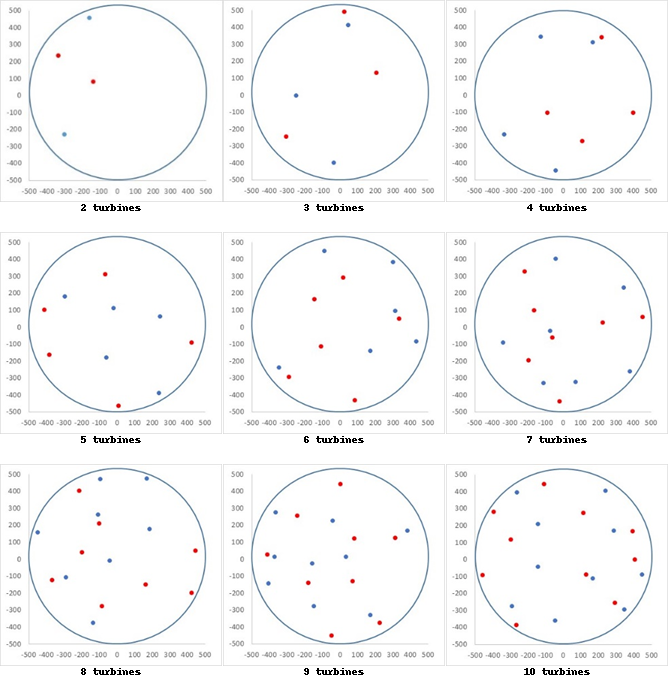
\includegraphics[width=\textwidth]{Layout_500m_wind data set I.png}
\caption{Archived layout visualizations for the 500~m farm under Wind Data Set I.}
\label{fig:layout500I}
\end{figure*}

\begin{figure*}[!t]
\centering
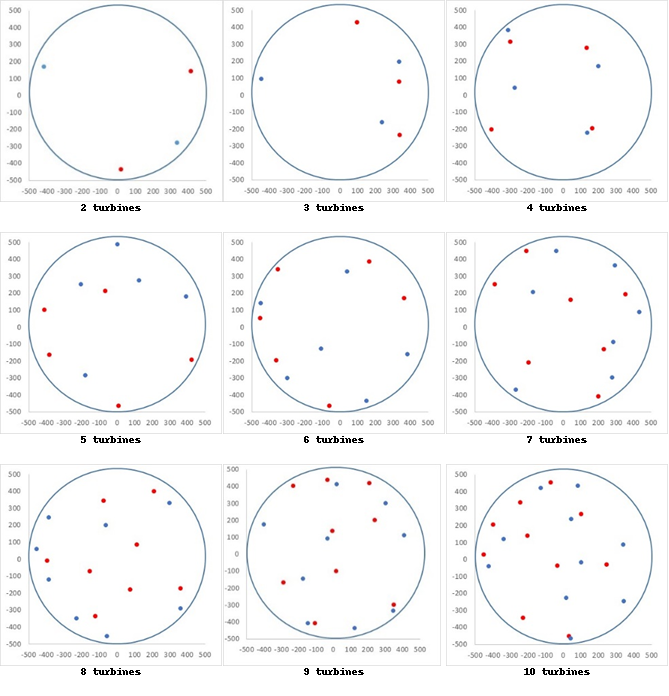
\includegraphics[width=\textwidth]{Layout_500m_wind data set II.png}
\caption{Archived layout visualizations for the 500~m farm under Wind Data Set II.}
\label{fig:layout500II}
\end{figure*}

\begin{figure*}[!t]
\centering
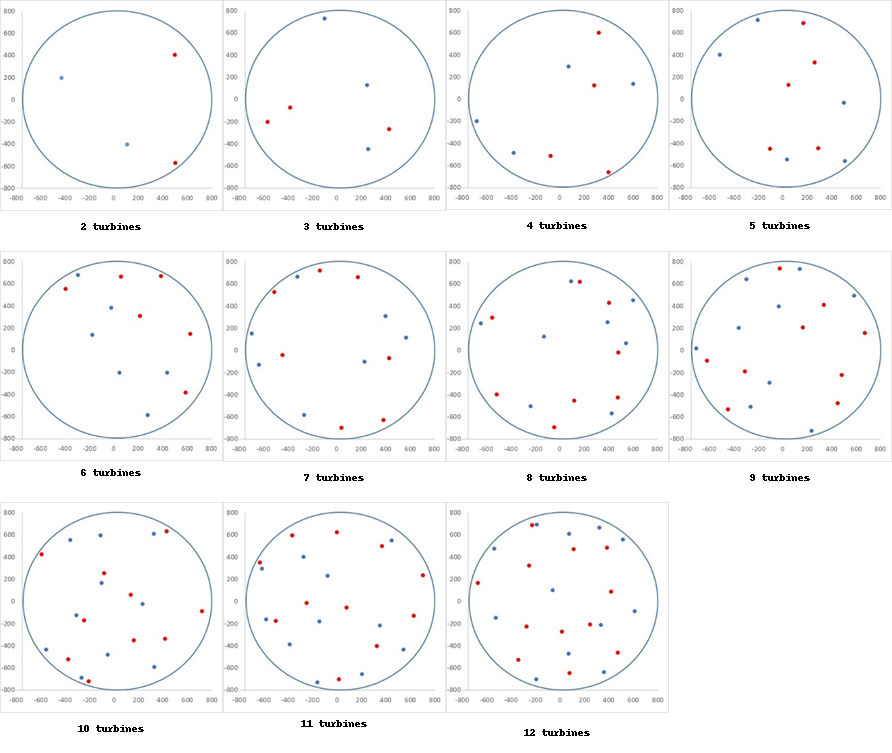
\includegraphics[width=\textwidth]{Layout_750m_wind data set I.png}
\caption{Archived layout visualizations for the 750~m farm under Wind Data Set I.}
\label{fig:layout750I}
\end{figure*}

\begin{figure*}[!t]
\centering
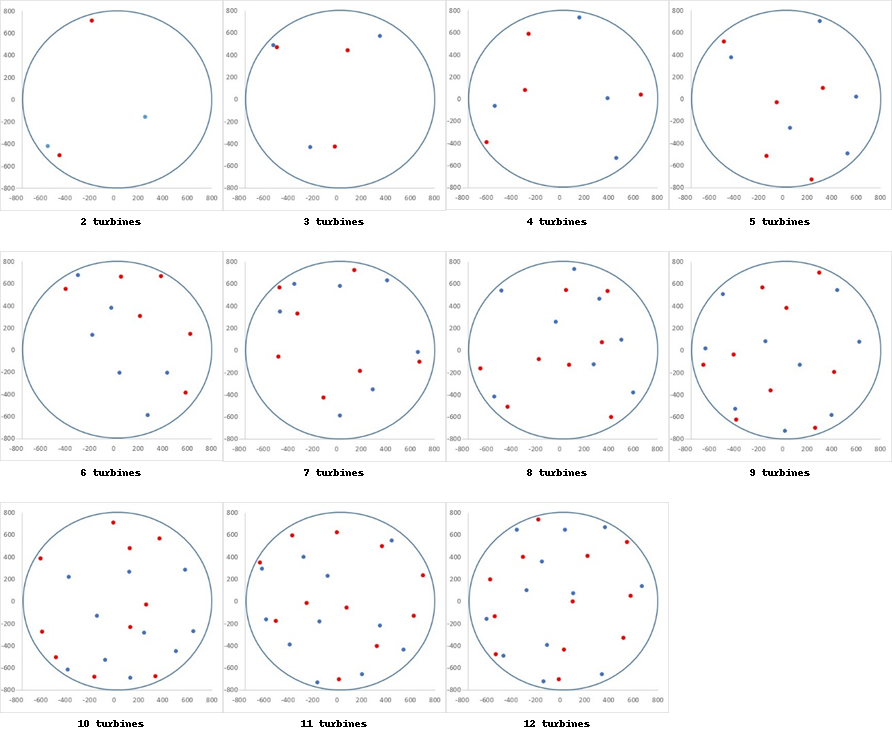
\includegraphics[width=\textwidth]{Layout_750m_wind data set II.png}
\caption{Archived layout visualizations for the 750~m farm under Wind Data Set II.}
\label{fig:layout750II}
\end{figure*}

\begin{figure*}[!t]
\centering
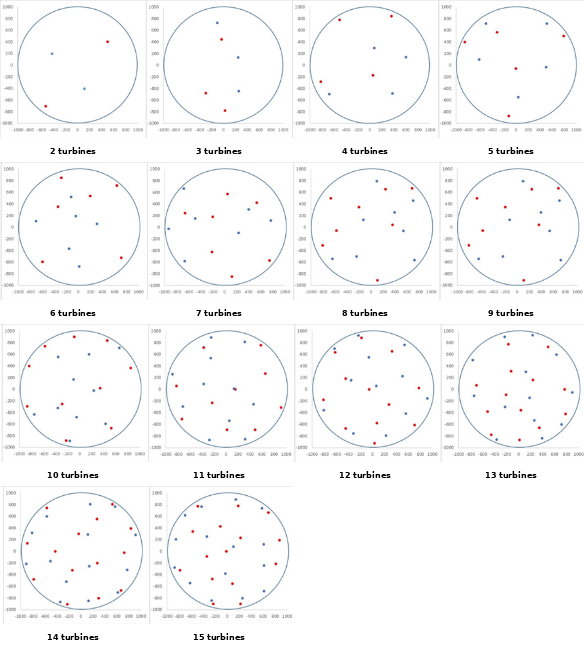
\includegraphics[width=\textwidth]{Layout_1000m_wind data set I.png}
\caption{Archived layout visualizations for the 1000~m farm under Wind Data Set I.}
\label{fig:layout1000I}
\end{figure*}

\begin{figure*}[!t]
\centering
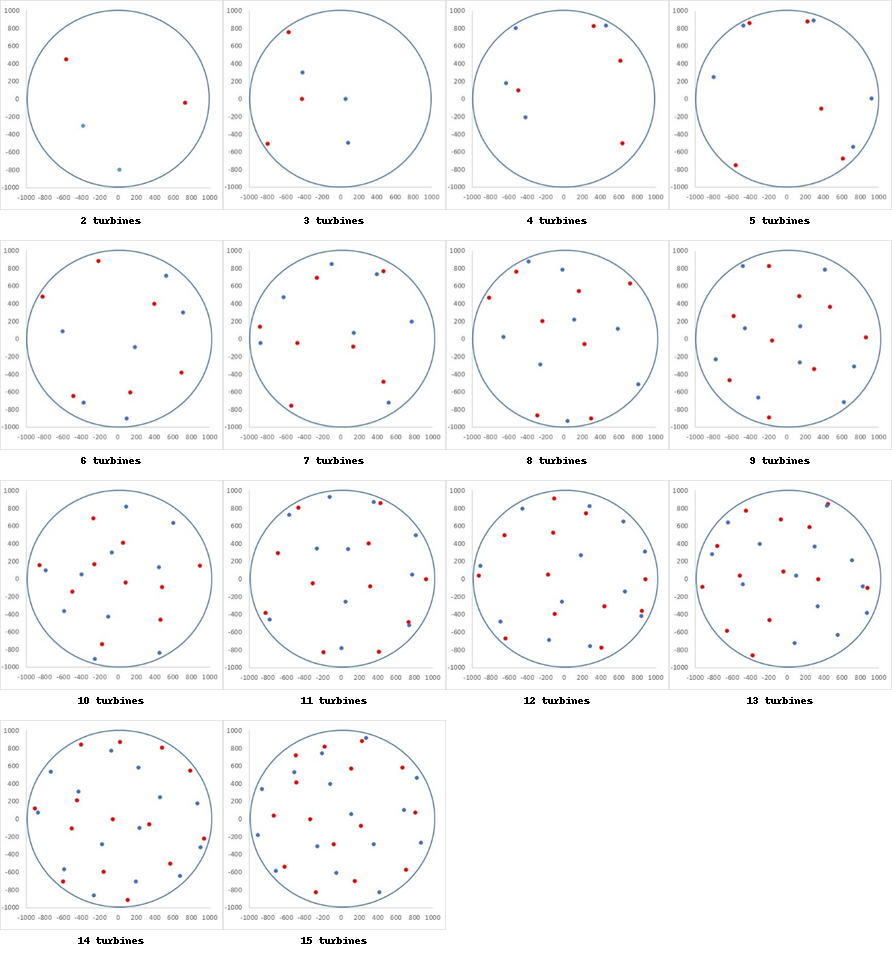
\includegraphics[width=\textwidth]{Layout_1000m_wind data set II.png}
\caption{Archived layout visualizations for the 1000~m farm under Wind Data Set II.}
\label{fig:layout1000II}
\end{figure*}


\section{Coordinates of the Best Follow-up Layouts}
\label{app:coordinates}
Table~\ref{tab:coords} lists the turbine coordinates (m, farm center at the origin) of the best LX-SSA layout among the 30 stored runs of each selected follow-up case. The coordinates of all 720 stored layouts (SSA, LX-SSA, PSO and DE) and the best layout of every algorithm are provided as machine-readable files with the revision. Every listed layout satisfies the circular boundary and the 308-m spacing, and its objective is reproduced by the independent evaluator of Section~\ref{sec:validation}.

\begin{table*}[!t]
\centering
\caption{Coordinates of the best LX-SSA layout in each selected follow-up case (benchmark objective and wake loss in objective units).}
\label{tab:coords}
\footnotesize\setlength{\tabcolsep}{3pt}
\begin{tabular}{cccccc l}
\toprule
DS & Radius (m) & $N$ & Seed & Objective & Wake loss & Coordinates $(\rho_i,\sigma_i)$ (m) \\
\midrule
1 & 500 & 4 & 6 & 56112.41 & 70.54 & (196.0, -400.4); (-279.0, 410.2); (-449.9, -177.2); (385.6, 318.3) \\
\midrule
1 & 750 & 8 & 1 & 111936.73 & 429.17 & (-681.8, -15.6); (-438.6, -516.0); (218.1, 154.6); (654.0, 343.4) \\
 & & & & & & (437.5, -505.9); (-428.3, 524.3); (-25.5, -663.1); (-11.5, 490.3) \\
\midrule
1 & 1000 & 8 & 13 & 112092.10 & 273.79 & (72.4, 277.4); (985.3, -119.6); (-728.9, 674.8); (431.5, -214.8) \\
 & & & & & & (-719.0, -268.9); (-325.8, -943.2); (-132.6, -205.3); (681.2, 699.8) \\
\midrule
2 & 500 & 4 & 10 & 29151.23 & 110.29 & (-75.0, 493.7); (-62.1, -481.3); (181.8, -211.8); (-417.8, 133.9) \\
\midrule
2 & 750 & 8 & 23 & 57331.96 & 1191.07 & (608.3, 144.1); (-551.5, 479.6); (22.0, -741.0); (133.4, 737.1) \\
 & & & & & & (-167.3, -179.1); (545.1, 466.6); (580.4, -182.3); (-718.3, -215.8) \\
\midrule
2 & 1000 & 8 & 17 & 58117.49 & 405.54 & (524.2, -325.3); (-576.4, -335.7); (-633.4, -663.6); (550.0, -665.6) \\
 & & & & & & (282.8, 911.8); (684.2, -10.8); (-357.4, 261.6); (-510.2, 702.3) \\
\bottomrule
\end{tabular}
\end{table*}


\vspace{1em}
\noindent\textbf{Compliance with Ethical Standards}

\vspace{0.5em}
\noindent\textbf{Conflict of Interest:} The authors declare that they have no conflict of interest.

\vspace{0.5em}
\noindent\textbf{Ethical Approval:} This article does not contain any studies with human participants or animals performed by any of the authors.

\vspace{0.5em}
\noindent\textbf{Informed Consent:} Not applicable.

\begin{thebibliography}{99}

\bibitem{Mosetti1994}
Mosetti, G., Poloni, C. and Diviacco, B. (1994). Optimization of wind turbine positioning in large windfarms by means of a genetic algorithm, \textit{J. Wind Engineering and Industrial Aerodynamics} \textbf{51}(1), 105-116.

\bibitem{Grady2005}
Grady, S., Hussaini, M. and Abdullah, M.M. (2005). Placement of wind turbines using genetic algorithms, \textit{Renewable Energy} \textbf{30}(2), 259-270.

\bibitem{Ozturk2004}
Ozturk, U.A. and Norman, B.A. (2004). Heuristic methods for wind energy conversion system positioning, \textit{Electric Power Systems Research} \textbf{70}(3), 179-185.

\bibitem{Lackner2007}
Lackner, M.A. and Elkinton, C.N. (2007). An analytical framework for offshore wind farm layout optimization, \textit{Wind Engineering} \textbf{31}(1), 17-31.

\bibitem{Mora2007}
Mora, J.C., Baron, L.M.C., Santos J.M.R. and Payan, M.B. (2007). An evolutive algorithm for wind farm optimal design, \textit{Neurocomputing} \textbf{70}(16), 2651-2658.

\bibitem{Huang2007}
Huang, H.S. (2007). Distributed genetic algorithm for optimization of wind farm annual profits, 14th International Conference on Intelligent System Applications to Power Systems, ISAP 2007, Taiwan, IEEE, 1-6.

\bibitem{Elkinton2008}
Elkinton, C.N., Manwell, J.F. and McGowan, J.G. (2008). Algorithms for offshore wind farm layout optimization, \textit{Wind Engineering} \textbf{32}(1), 67–84.

\bibitem{Bilbao2009}
Bilbao, M. and Alba, E. (2009). Simulated annealing for optimization of wind farm annual profit, 2nd International Symposium on Logistics and Industrial Informatics, IEEE, Austria, 1-5.

\bibitem{Rivas2009}
Rivas, R.A., Clausen, J., Hansen, K.S. and Jensen, L.E. (2009). Solving the turbine positioning problem for large offshore wind farms by simulated annealing, \textit{Wind Engineering} \textbf{33}(3), 287-297.

\bibitem{Emami2010}
Emami, A. and Noghreh, P. (2010). New approach on optimization in placement of wind turbines within wind farm by genetic algorithms, \textit{Renewable Energy} \textbf{35}(7), 1559-1564.

\bibitem{Sisbot2010}
Sisbot S., Turgut, O., Tunç, M. and Çamdalı, U.(2010). Optimal positioning of wind turbines on gokçeada using multi-objective genetic algorithm, \textit{Wind Energy} \textbf{13}(4), 297-306.

\bibitem{Kusiak2010}
Kusiak, A. and Song, Z. (2010). Design of wind farm layout for maximum wind energy capture, \textit{Renewable Energy} \textbf{35}(3), 685-694.

\bibitem{Eroglu2012}
Eroglu, Y. and Seckiner, S.U. (2012). Design of wind farm layout using ant colony algorithm, \textit{Renewable Energy} \textbf{44}, 53-62.

\bibitem{Eroglu2013}
Eroglu, Y. and Seckiner, S.U. (2013). Wind farm layout optimization using particle filtering approach, \textit{Renewable Energy} \textbf{58}, 95-107.

\bibitem{Samorani2013}
Samorani, M. (2013). The wind farm layout optimization problem, in: \textit{Handbook of Wind Power Systems}, Springer, 21-38.

\bibitem{Bansal2017}
Bansal, J.C. and Farswan, P. (2017). Wind farm layout using Biogeography Based Optimization, \textit{Renewable Energy} \textbf{107}, 386-402.

\bibitem{Ju2019}
Ju, X. and Liu. F. (2019). Wind farm layout optimization using self-informed genetic algorithm with information guided exploitation, \textit{Applied Energy} \textbf{248}, 429-445.

\bibitem{Jin2019}
Jin, R., Hou, P., Yang, G., Qi, Y., Chen, C. and Chen, Z. (2019). Cable routing optimization for offshore wind power plants via wind scenarios considering power loss cost model, \textit{Applied Energy} \textbf{254}. \url{https://doi.org/10.1016/j.apenergy.2019.113719}

\bibitem{Dhiman2020}
Dhiman, H.S., Deb, D. and Foley, A.M. (2020). Lidar assisted wake redirection in wind farms: A data driven approach, \textit{Renewable Energy} \textbf{152}, 484-493.

\bibitem{Nagpal2021}
Nagpal, S.V., Liu, M.V. and Anderson, C.L. (2021). A comparison of deterministic refinement techniques for wind farm layout optimization, \textit{Renewable Energy} \textbf{168}, 581-592.

\bibitem{Bai2022}
Bai, F., Ju, X., Wang, S., Zhou, W. and Liu, F. (2022). Wind farm layout optimization using adaptive evolutionary algorithm with Monte Carlo Tree Search reinforcement learning, \textit{Energy Conversion and Management} \textbf{252}. \url{https://doi.org/10.1016/j.enconman.2021.115047}

\bibitem{Cazzaro2022}
Cazzaro, D. and Pisinger, D. (2022). Variable neighborhood search for large offshore wind farm layout optimization, \textit{Computers \& Operations Research} \textbf{138}. \url{https://doi.org/10.1016/j.cor.2021.105588}

\bibitem{Jensen1983}
Jensen, N. O. (1983). A Note on Wind Generator Interaction, Risø National Laboratory.

\bibitem{Katic1986}
Katic, I., Højstrup, J. and Jensen, N.O. (1986). A simple model for cluster efficiency, in: \textit{European Wind Energy Association Conference and Exhibition}, 407-410.

\bibitem{Stroock1999}
Stroock, D.W. (1999). A concise introduction to the theory of integration, Springer Science \& Business Media, 1999.

\bibitem{Mirjalili2017}
Mirjalili, S., Gandomi, A.H., Mirjalili, S.Z., Saremi, S., Faris, H., \& Mirjalili, S.M. (2017). Salp Swarm Algorithm: A bio-inspired optimizer for engineering design problems. \textit{Advances in Engineering Software} \textbf{114}, 163-191.

\bibitem{Srikakulapu2018}
Srikakulapu, R. and Vinatha, U. (2018). Optimized design of collector topology for offshore wind farm based on ant colony optimization with multiple travelling salesman problem, \textit{Journal of Modern Power Systems and Clean Energy} \textbf{6}, 1181--1192. doi:10.1007/s40565-018-0386-4.

\bibitem{Hou2019}
Hou, P., Zhu, J., Ma, K., et al. (2019). A review of offshore wind farm layout optimization and electrical system design methods, \textit{Journal of Modern Power Systems and Clean Energy} \textbf{7}(4), 975--986. doi:10.1007/s40565-019-0544-7.

\bibitem{Asaah2021}
Asaah, P., Hao, L. and Ji, J. (2021). Optimal placement of wind turbines in wind farm layout using particle swarm optimization, \textit{Journal of Modern Power Systems and Clean Energy} \textbf{9}(2), 367--375. doi:10.35833/MPCE.2019.000087.

\bibitem{Solanki2023}
Solanki, P. and Deep, K. (2023). Laplacian Salp Swarm Algorithm for continuous optimization, \textit{International Journal of System Assurance Engineering and Management}. doi:10.1007/s13198-023-01935-y.

\bibitem{Deep2007}
Deep, K. and Thakur, M. (2007). A new crossover operator for real-coded genetic algorithms. \textit{Applied Mathematics and Computation} \textbf{188}, 895-911.



\bibitem{SolankiQA2024}
Solanki, P. and Deep, K. (2024). Quadratic approximation salp swarm algorithm for function optimization, \textit{OPSEARCH} \textbf{61}(1), 282--314. doi:10.1007/s12597-023-00682-9.

\bibitem{Quaeghebeur2021}
Quaeghebeur, E., Bos, R. and Zaaijer, M.B. (2021). Wind farm layout optimization using pseudo-gradients, \textit{Wind Energy Science} \textbf{6}, 815--839. doi:10.5194/wes-6-815-2021.

\bibitem{Tao2020}
Tao, S., Xu, Q., Feij\'oo, A., Zheng, G. and Zhou, J. (2020). Wind farm layout optimization with a three-dimensional Gaussian wake model, \textit{Renewable Energy} \textbf{159}, 553--569. doi:10.1016/j.renene.2020.06.003.

\bibitem{Yang2023}
Yang, K., Deng, X., Ti, Z., Yang, S., Huang, S. and Wang, Y. (2023). A data-driven layout optimization framework of large-scale wind farms based on machine learning, \textit{Renewable Energy} \textbf{218}, 119240. doi:10.1016/j.renene.2023.119240.

\bibitem{Wang2024}
Wang, Z., Tu, Y., Zhang, K., Han, Z., Cao, Y. and Zhou, D. (2024). An optimization framework for wind farm layout design using CFD-based Kriging model, \textit{Ocean Engineering} \textbf{293}, 116644. doi:10.1016/j.oceaneng.2023.116644.

\bibitem{Yang2024}
Yang, S., Deng, X. and Yang, K. (2024). Machine-learning-based wind farm optimization through layout design and yaw control, \textit{Renewable Energy} \textbf{224}, 120161. doi:10.1016/j.renene.2024.120161.

\bibitem{Li2025}
Li, P., Che, Y., Hua, A., Wang, L., Zheng, M. and Guo, X. (2025). A data-physics hybrid-driven layout optimization framework for large-scale wind farms, \textit{Applied Energy} \textbf{392}, 125908. doi:10.1016/j.apenergy.2025.125908.

\bibitem{Cao2022}
Cao, L., Ge, M., Gao, X., Du, B., Li, B., Huang, Z. and Liu, Y. (2022). Wind farm layout optimization to minimize the wake induced turbulence effect on wind turbines, \textit{Applied Energy} \textbf{323}, 119599. doi:10.1016/j.apenergy.2022.119599.

\bibitem{PyWake}
DTU Wind Energy. PyWake: an open-source wind farm simulation tool, Python package \texttt{py\_wake} version 2.6.20 (Horns Rev~1 site data, \texttt{py\_wake/examples/data/hornsrev1.py}), MIT License. \url{https://gitlab.windenergy.dtu.dk/TOPFARM/PyWake}.

\bibitem{Carrillo2013}
Carrillo, C., Obando Monta\~no, A.F., Cidr\'as, J. and D\'iaz-Dorado, E. (2013). Review of power curve modelling for wind turbines, \textit{Renewable and Sustainable Energy Reviews} \textbf{21}, 572--581. doi:10.1016/j.rser.2013.01.012.

\bibitem{Bastankhah2014}
Bastankhah, M. and Port\'e-Agel, F. (2014). A new analytical model for wind-turbine wakes, \textit{Renewable Energy} \textbf{70}, 116--123. doi:10.1016/j.renene.2014.01.029.

\bibitem{Demsar2006}
Dem\v{s}ar, J. (2006). Statistical comparisons of classifiers over multiple data sets, \textit{Journal of Machine Learning Research} \textbf{7}, 1--30.

\bibitem{Holm1979}
Holm, S. (1979). A simple sequentially rejective multiple test procedure, \textit{Scandinavian Journal of Statistics} \textbf{6}(2), 65--70.

\bibitem{Vargha2000}
Vargha, A. and Delaney, H.D. (2000). A critique and improvement of the CL common language effect size statistics of McGraw and Wong, \textit{Journal of Educational and Behavioral Statistics} \textbf{25}(2), 101--132.

\end{thebibliography}


\end{document}
